\documentclass[10pt]{article}
\usepackage{amsmath}
\usepackage{listings}
\usepackage{graphicx}
\usepackage{float}
\usepackage{tabularx}
\graphicspath{ {./images/} }
\begin{document}
{\centering
    CSU44061 Machine Learning - Week 4
    \par
    Samuel Petit - 17333946
    \par
    Dataset 1\# id:21-21-21-0 
    \par
    Dataset 2\# id:21--42--21-0  
    \par
}
\section*{Question i}
Code for all questions provided in the appendix.

\subsection*{Part a}
Using the first dataset. I used sklearn's PolynomialFeatures
to augment the two original features up to a provided polynomial order.

This is done as such:
\begin{lstlisting}
poly = PolynomialFeatures(<desired max order>)
X_poly = poly.fit_transform(<stack of features>)
\end{lstlisting}

I can then train Logistic Regression models for a range of
degrees in order to identify which one to use. I found that using a
range of degrees from 1 to 9 was appropriate as increasing the range further
would not provide more information when it comes to selecting an optimal value.
It is also worth noting that we keep track of each model's mean squared error
in order to use it within our plots. 

In terms of plotting this cross validation, I iterate through the set
of degrees, generate the features then keep a list of the scores for all
the trained models. The score is the mean accuracy of the model. The plot
then consists of an errorbar plot which uses the set of scores and degrees used.


Here is the code used to retrieve the scores:
\begin{lstlisting}
degrees = range(1, 10)
scores = []
temp = []
for degree in degrees:
    # Generate new features
    poly = PolynomialFeatures(degree)
    X_poly = poly.fit_transform(X)
    # Train the model
    model = LogisticRegression(penalty='l2')
                                    .fit(X_poly, y)
    # Keep the score of the model
    scores.append(model.score(X_poly, y))
    temp.append(mean_squared_error
                        (y, model.predict(X_poly)))
\end{lstlisting}

We then obtain the plot:
\begin{center}
    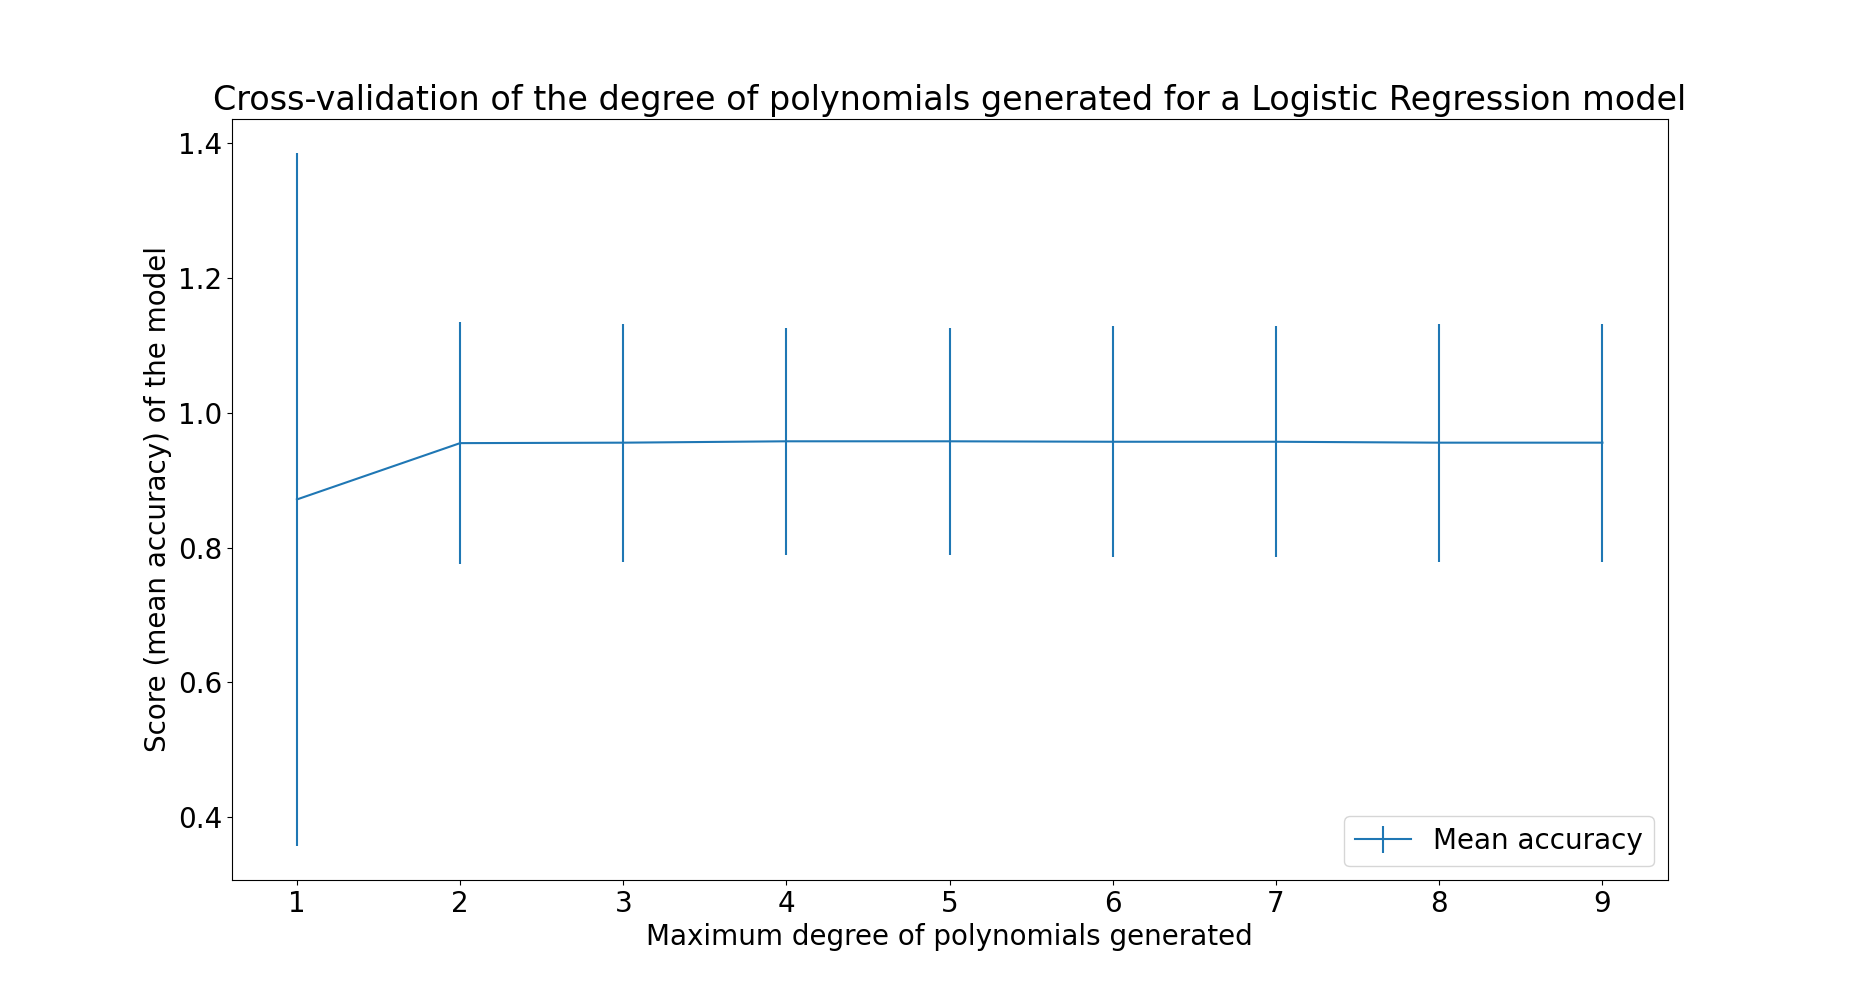
\includegraphics[scale=0.25]{ds_1_degree_cv.png}
\end{center}
\vspace{5mm} %5mm vertical space

We notice that once we get passed 2 degrees we pretty much get the same
score and mean squared error. We will then pick 2 as our maximum polynomial degree used,
this will reduce computing time and make sure that we get the best possible
predictions.

Let's compare predictions using a variety of interesting degrees, that is 1, 2 and 10
such as to get an idea of how our predictions are holding up against the provided data:

\begin{figure}[H]    
    \fbox{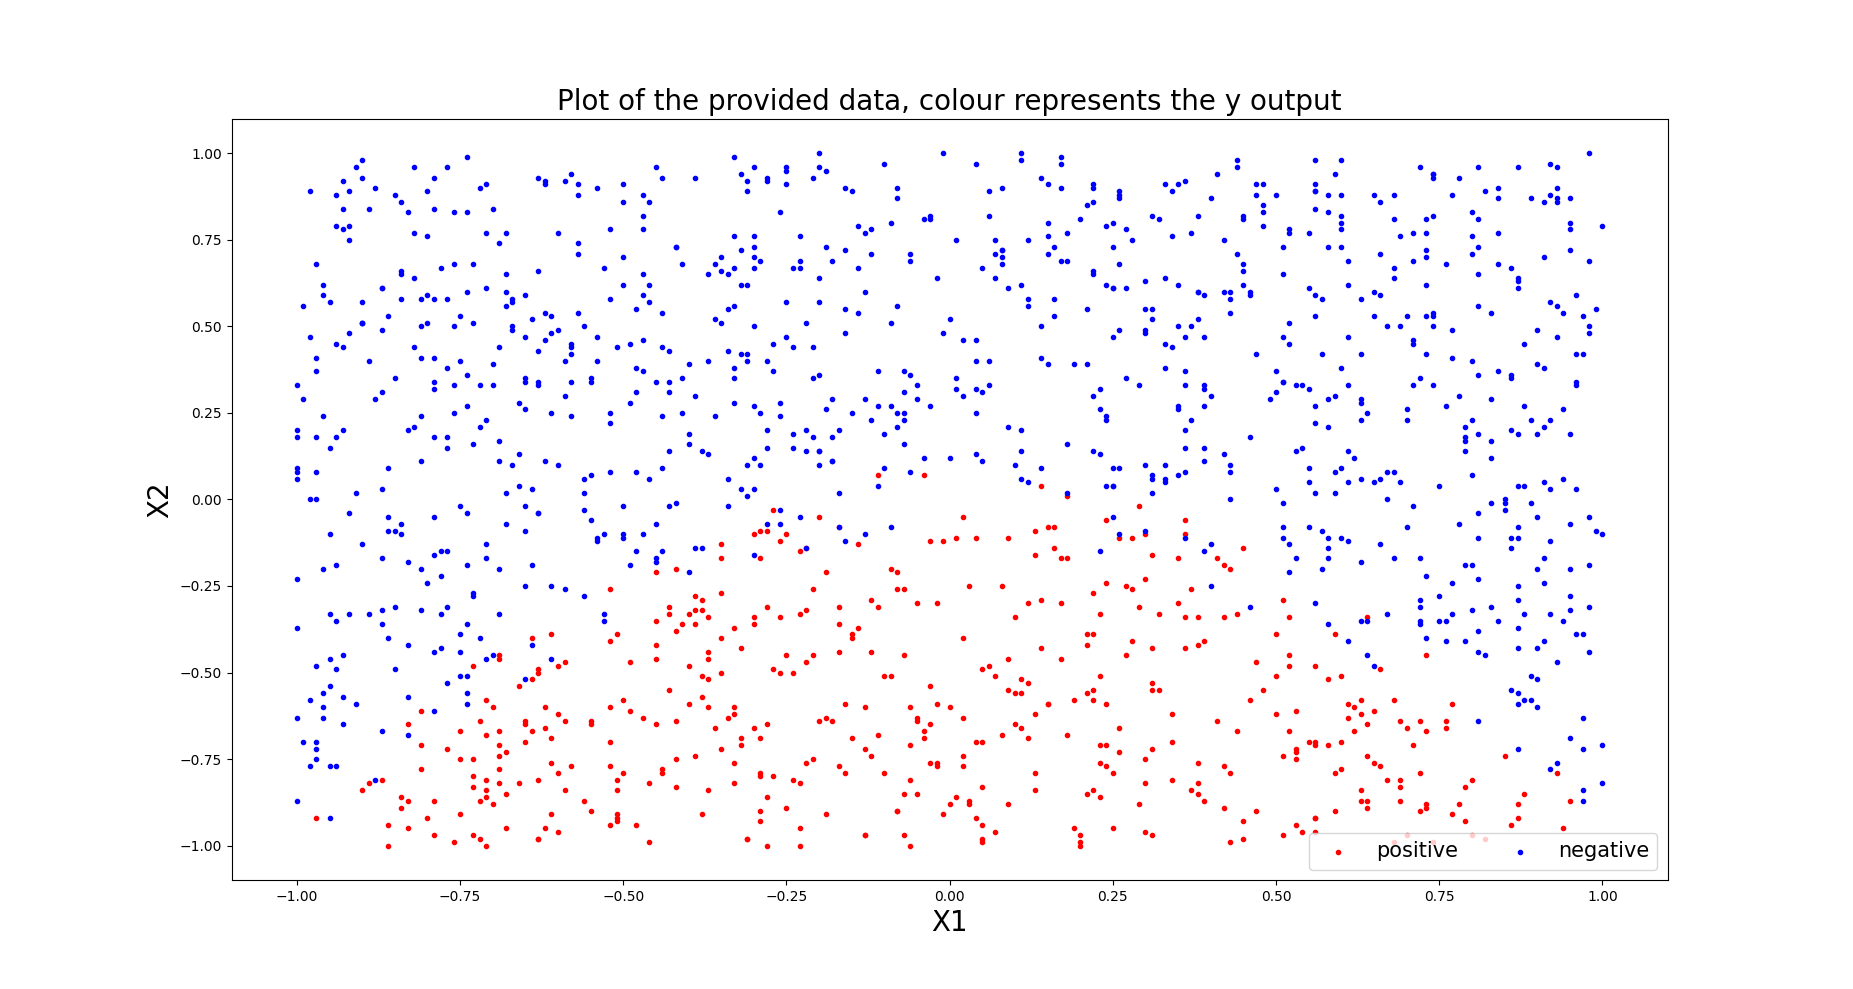
\includegraphics[scale=0.15]{Figure_1.png}}   
    \fbox{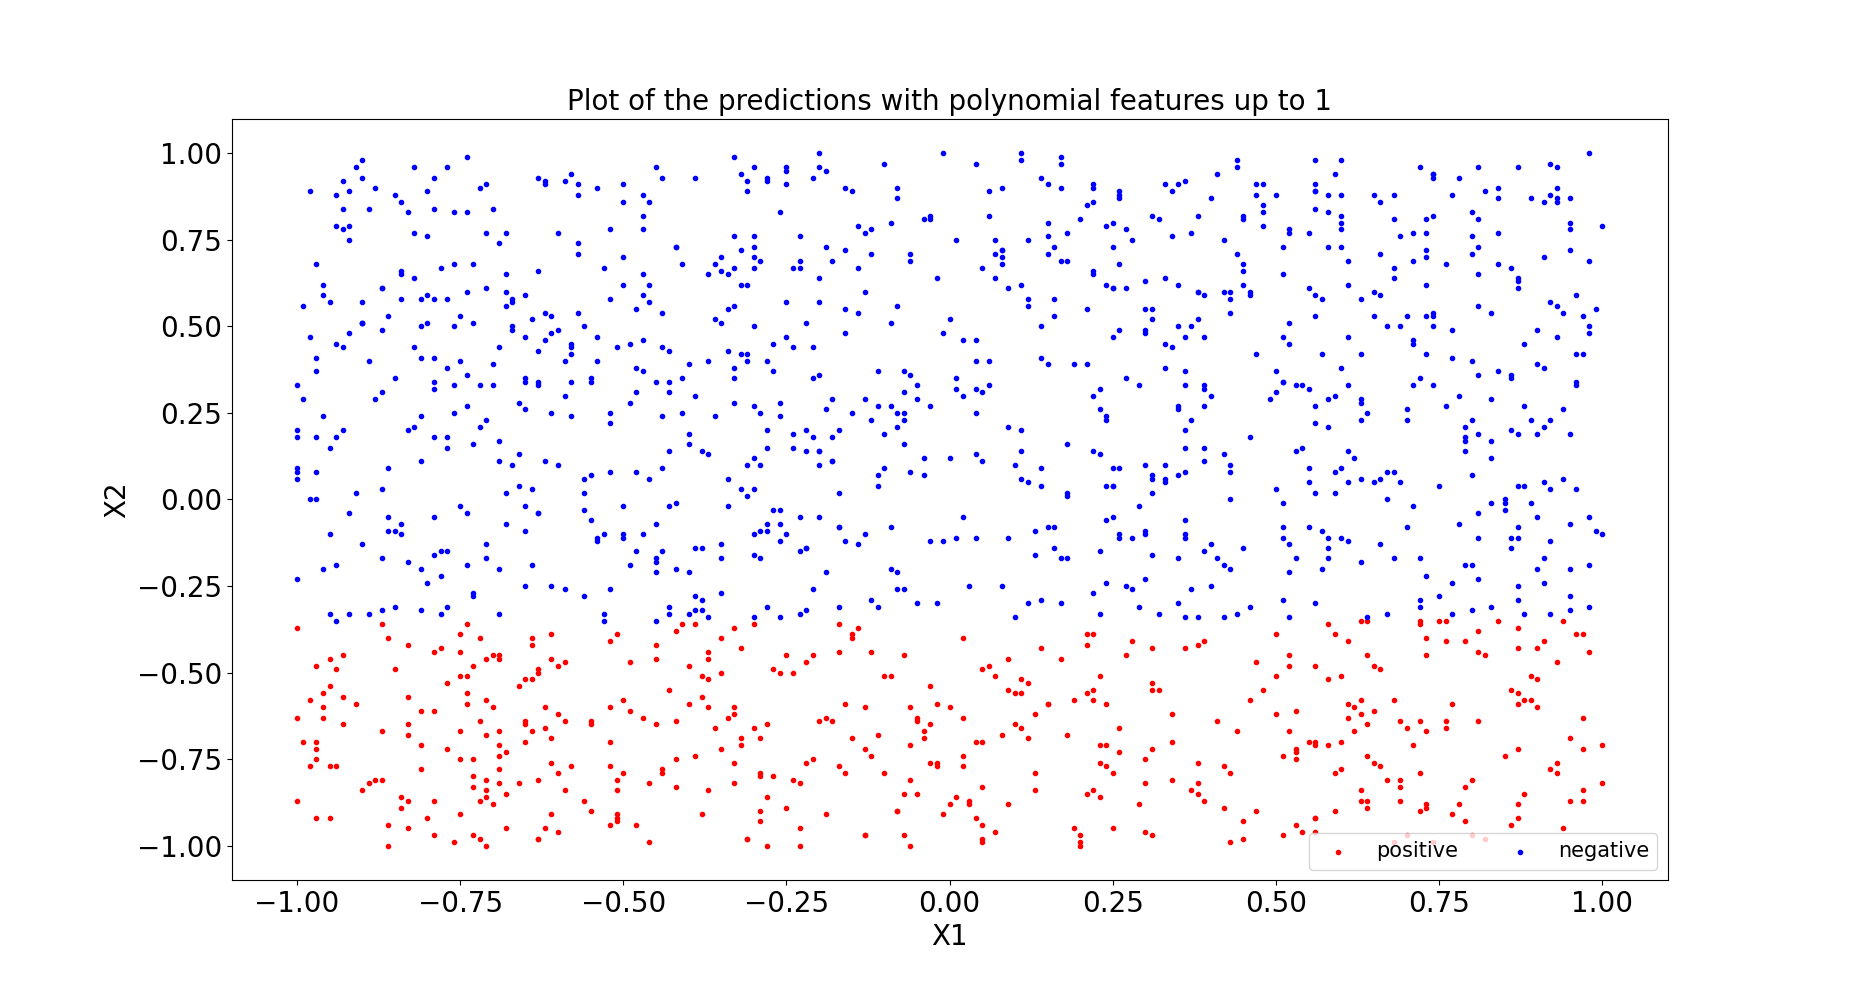
\includegraphics[scale=0.15]{ds_1_pred_d_1.png}}   
    \fbox{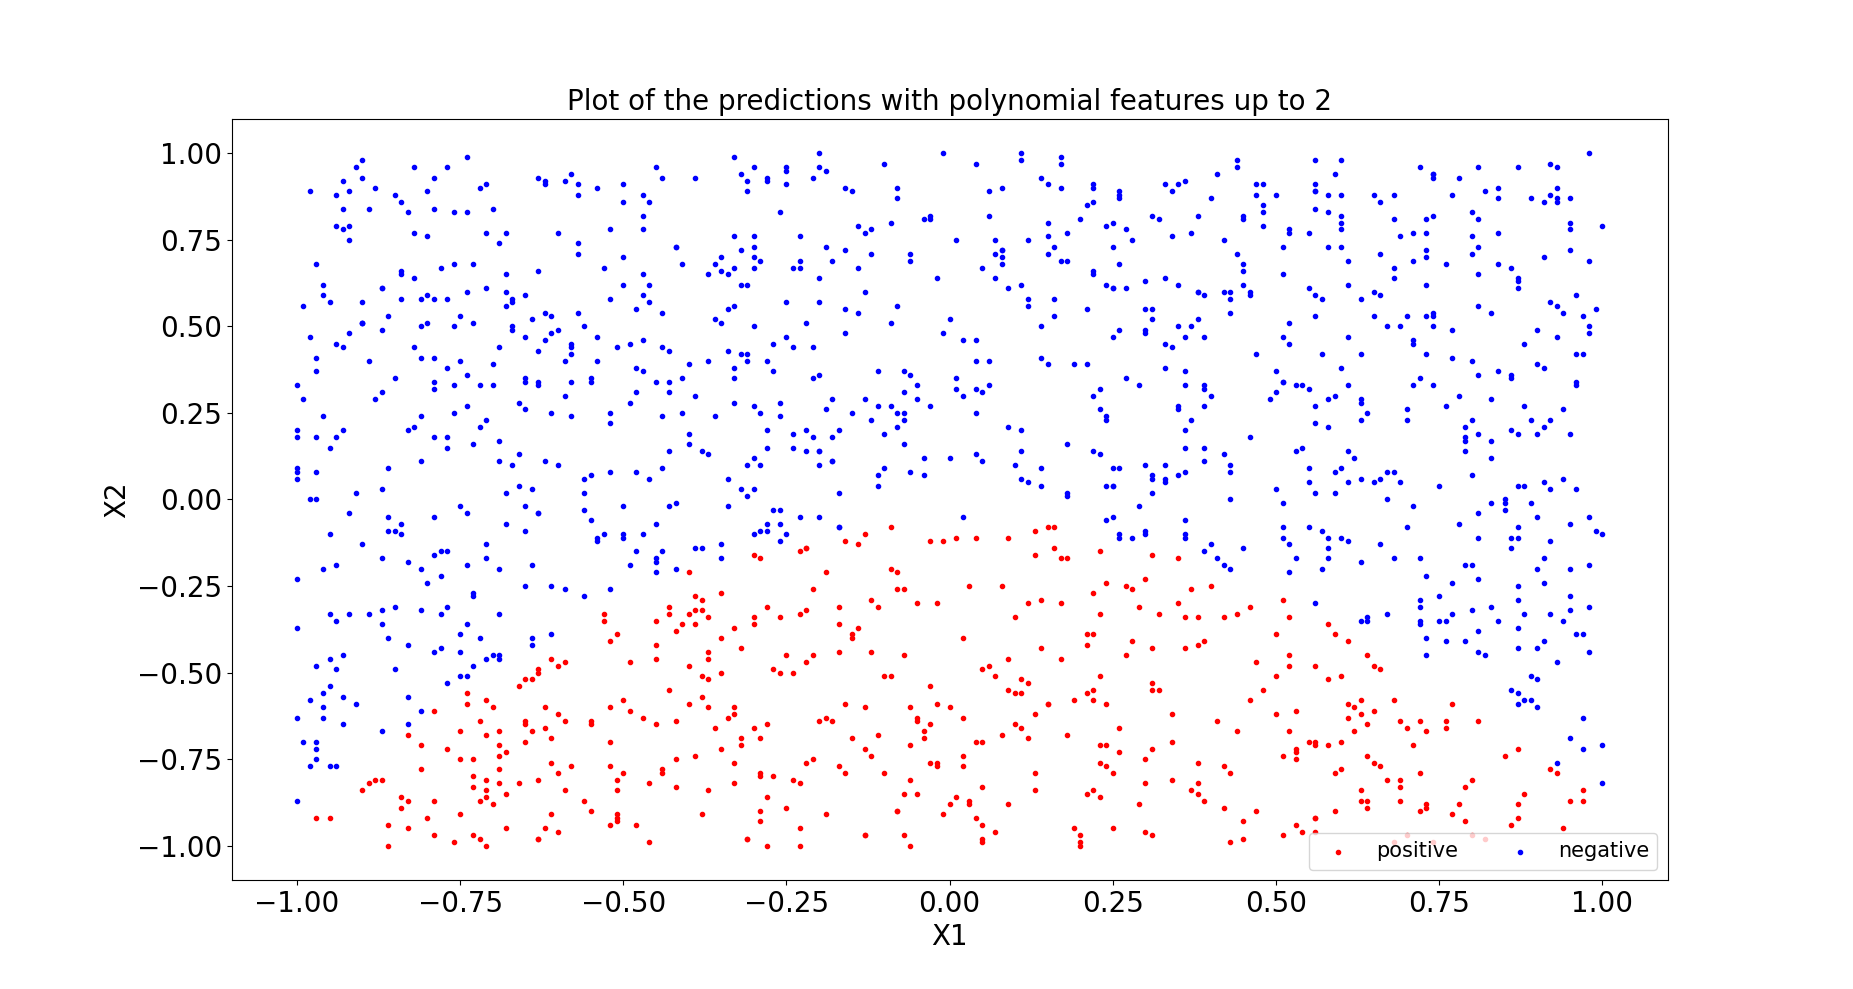
\includegraphics[scale=0.15]{ds_1_pred_d_2.png}}
    \fbox{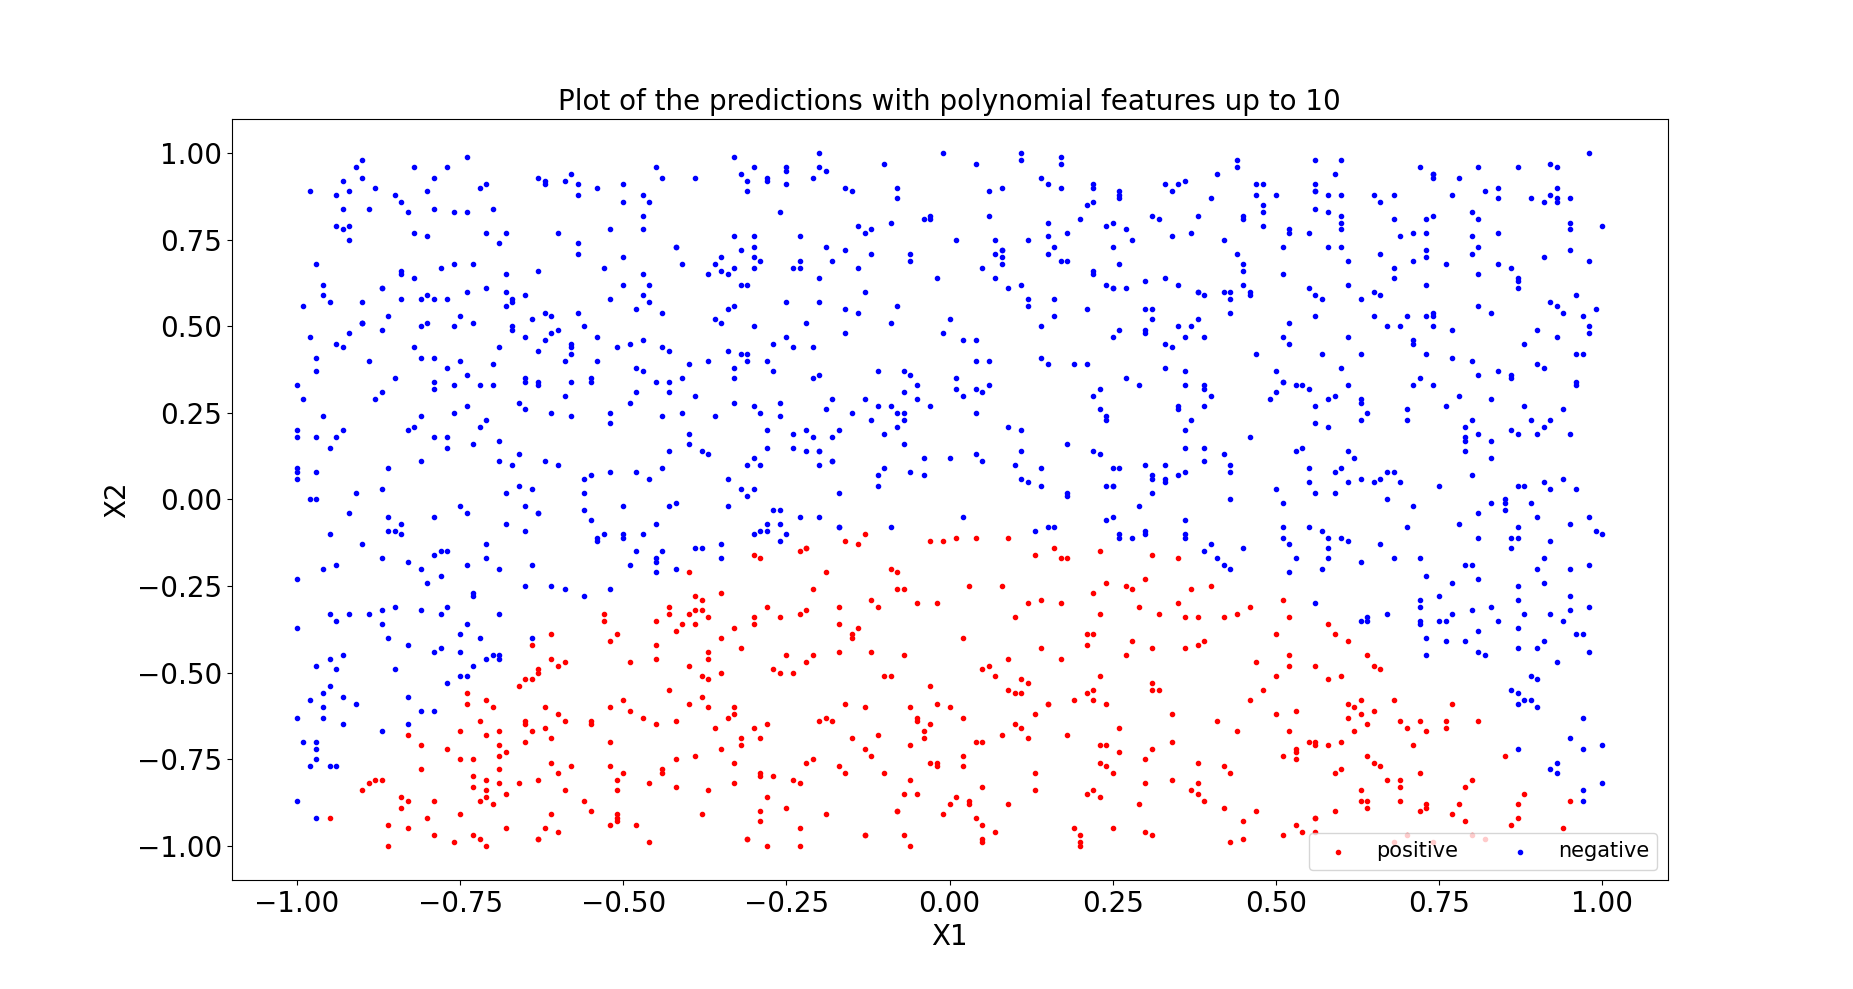
\includegraphics[scale=0.15]{ds_1_pred_d_10.png}}
\end{figure}

We can clearly see that what what we saw in the cross comparison graph
reflects in the model predictions. Using features of polynomial order
up to 1 yeilds a  fairly inacurrate model while degrees 2 and 10 are very
similar.

\vspace{5mm} %5mm vertical space

Let's now consider the C value. Using the exact same method as previously explained
but this time changing the value for C of our model, we obtain the following
cross validation graph. Note that for this one I chose a range going from
1 to 30 as once again, it includes all the data that is relevant to us in order
to make an educated decision as to deciding the C parameter. Increasing
the range would only make the computing time higher.

\begin{center}
    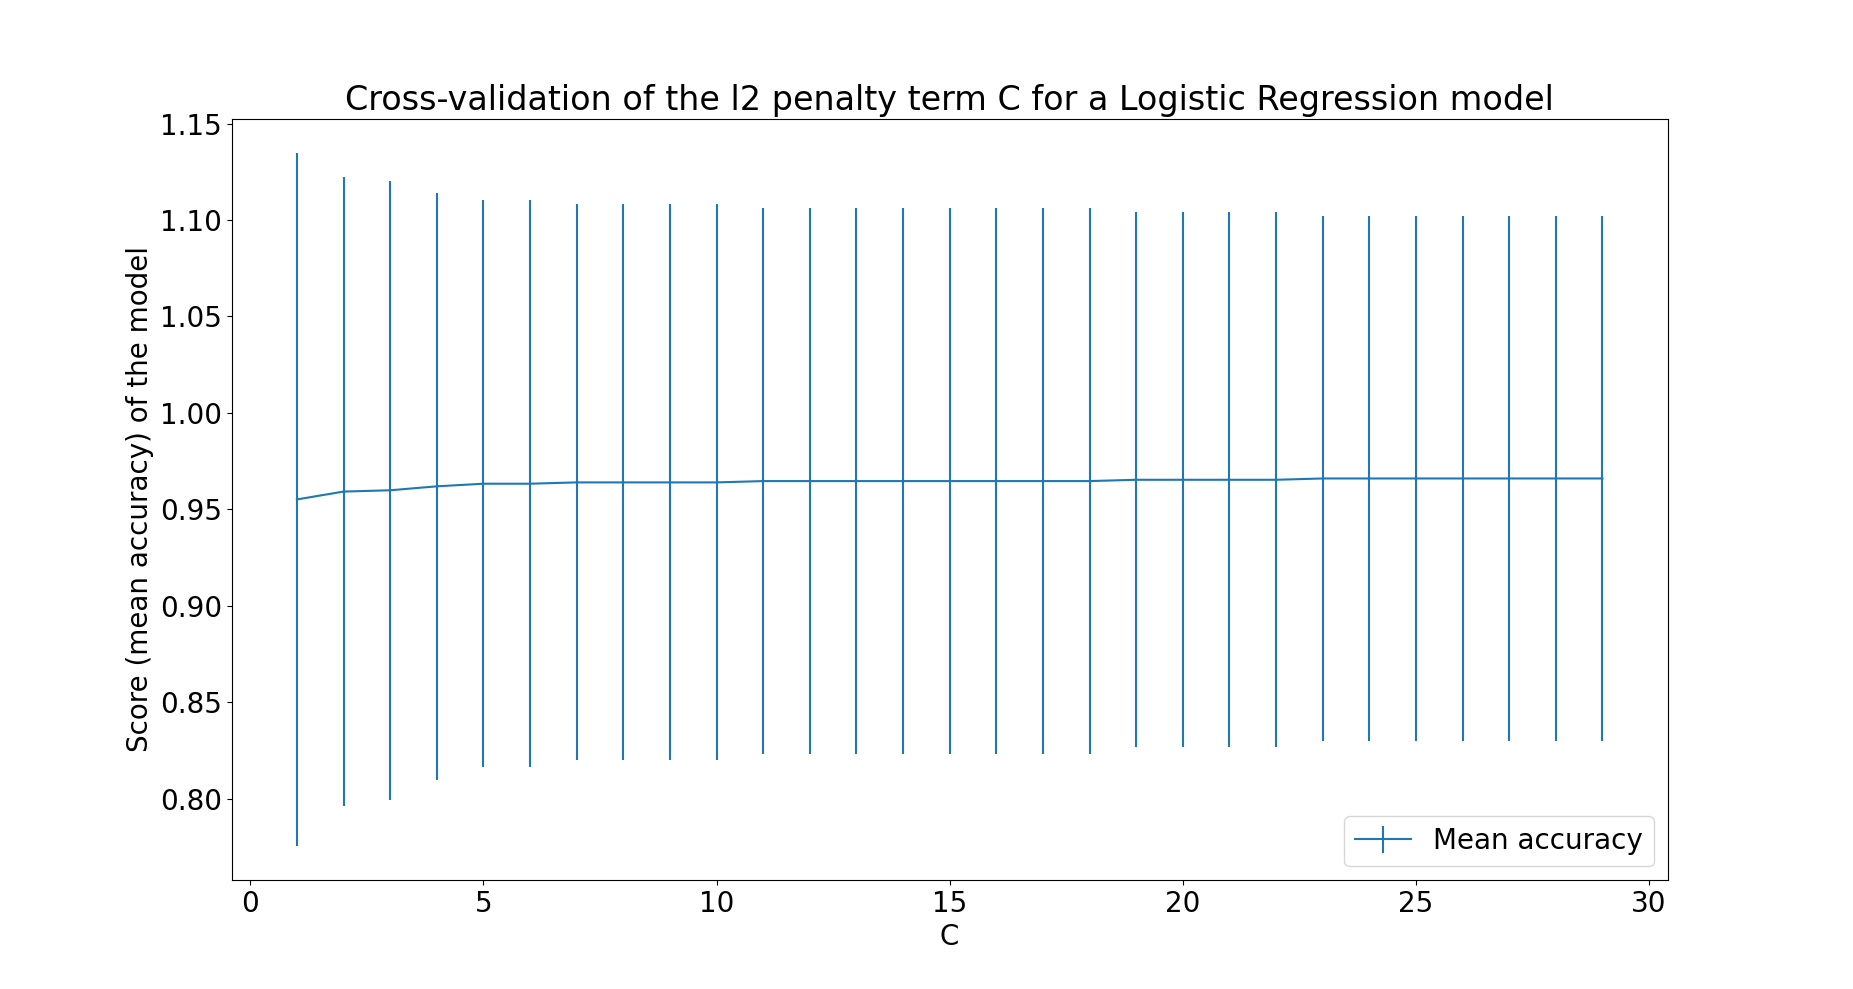
\includegraphics[scale=0.25]{ds_1_C_cv.png}
\end{center}
\vspace{5mm} %5mm vertical space

We find that most values for C yeild quite a similar score accuracy and mean squared
error. For this one, given that they are all quite similar with
the exception of $ C = 1 $, we pick the value $ C = 8 $ as it seems
to have a slightly lower variance and amongst the highest score.

Once again, plotting predictions for 3 of these models, using 3 values for C
at different point within the cross validation graph,
as well as the original data in order to compare them,
we obtain the following figure:

\begin{figure}[H]    
    \fbox{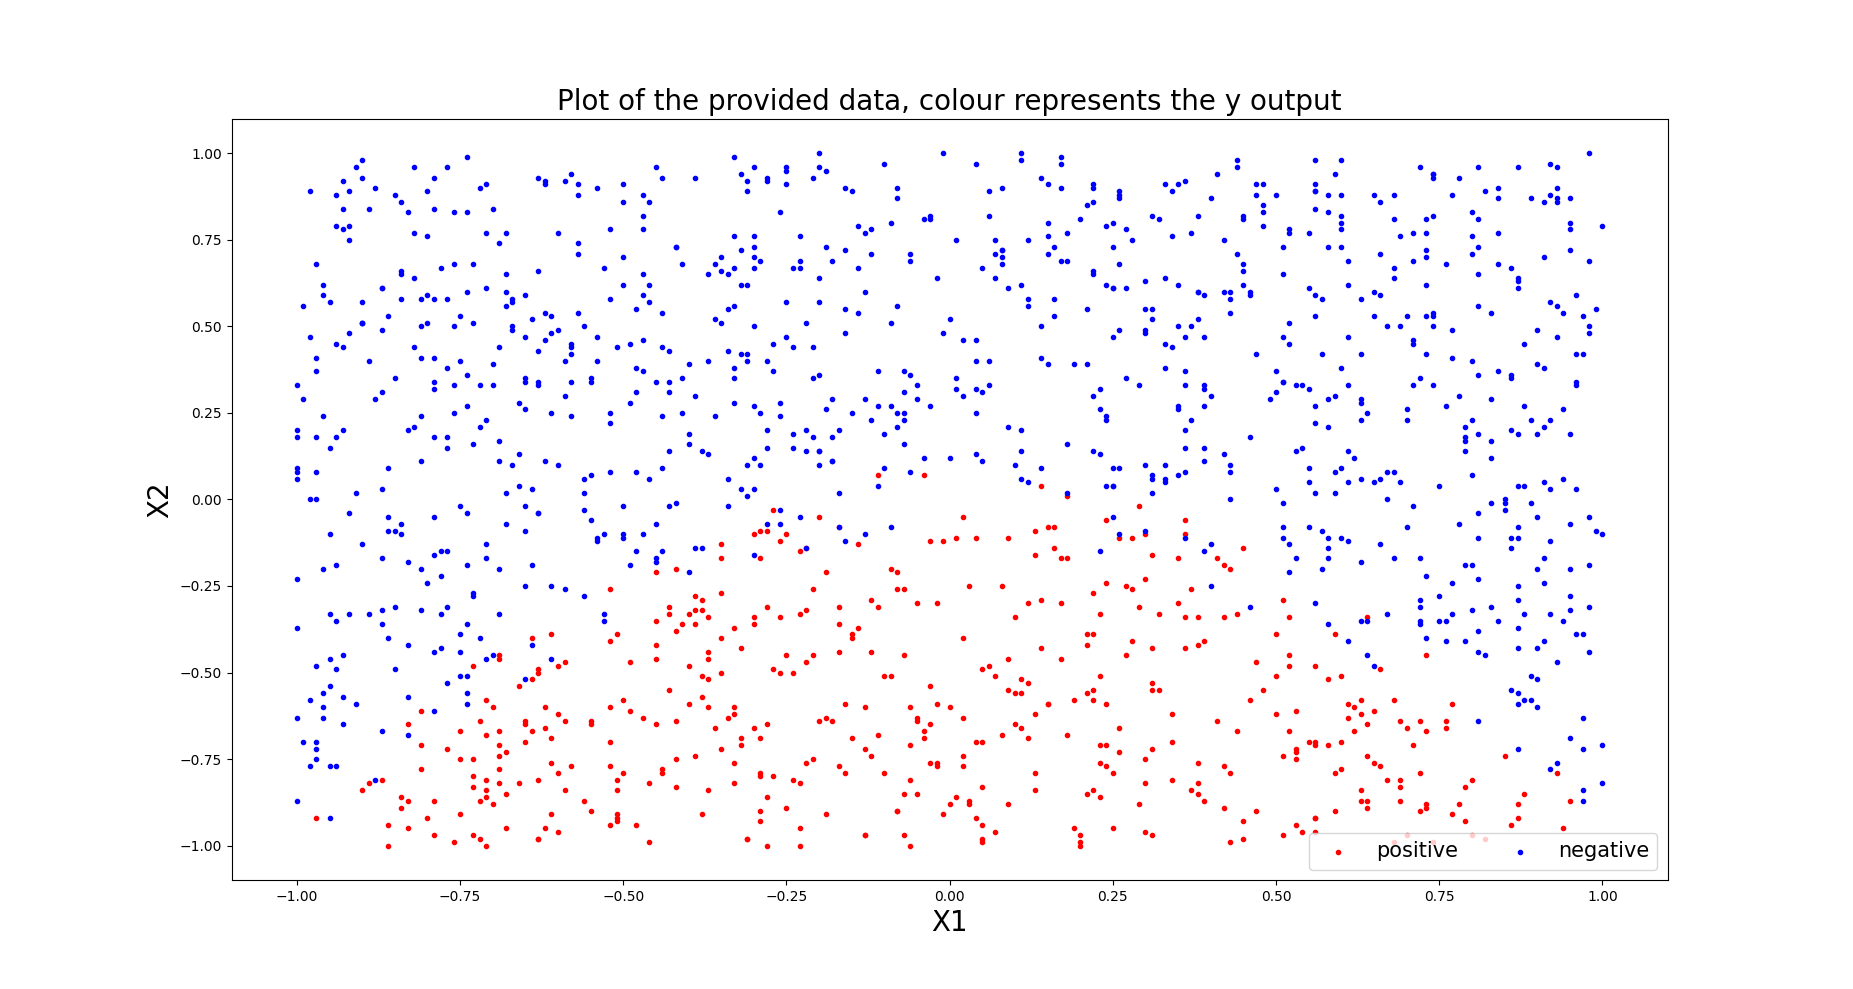
\includegraphics[scale=0.15]{Figure_1.png}}   
    \fbox{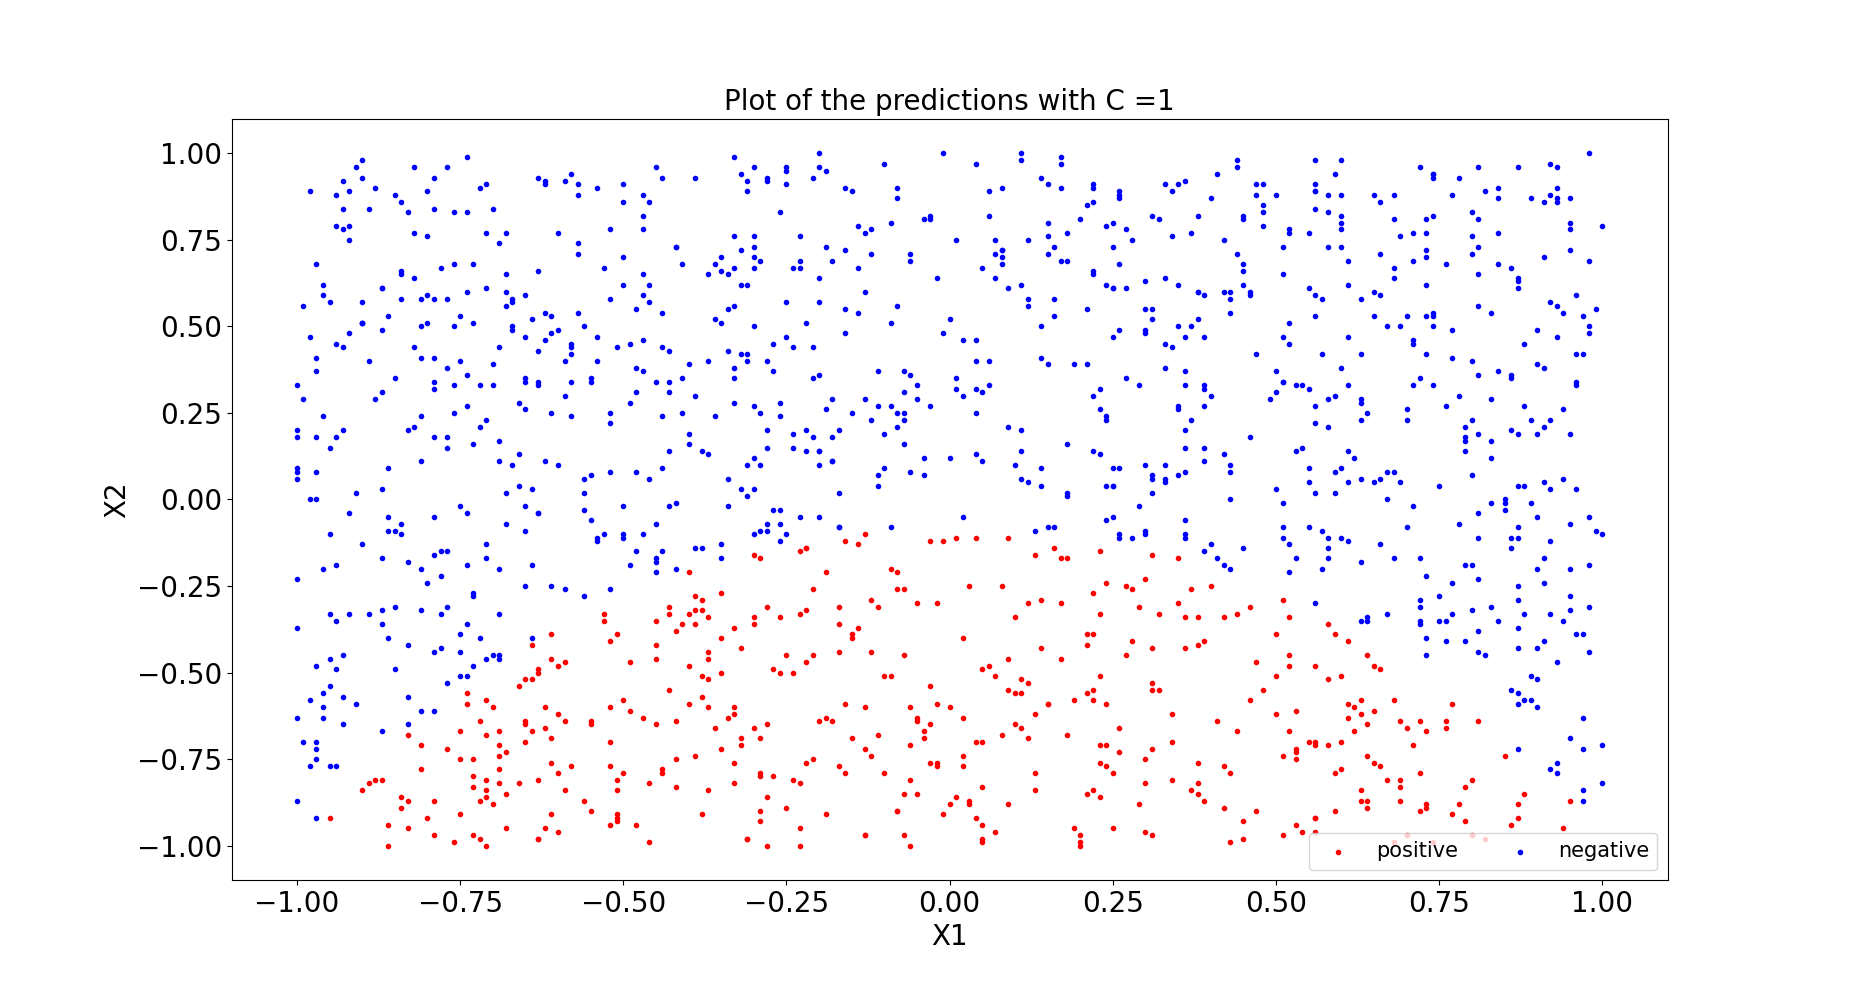
\includegraphics[scale=0.15]{ds_1_pred_c_1.png}}   
    \fbox{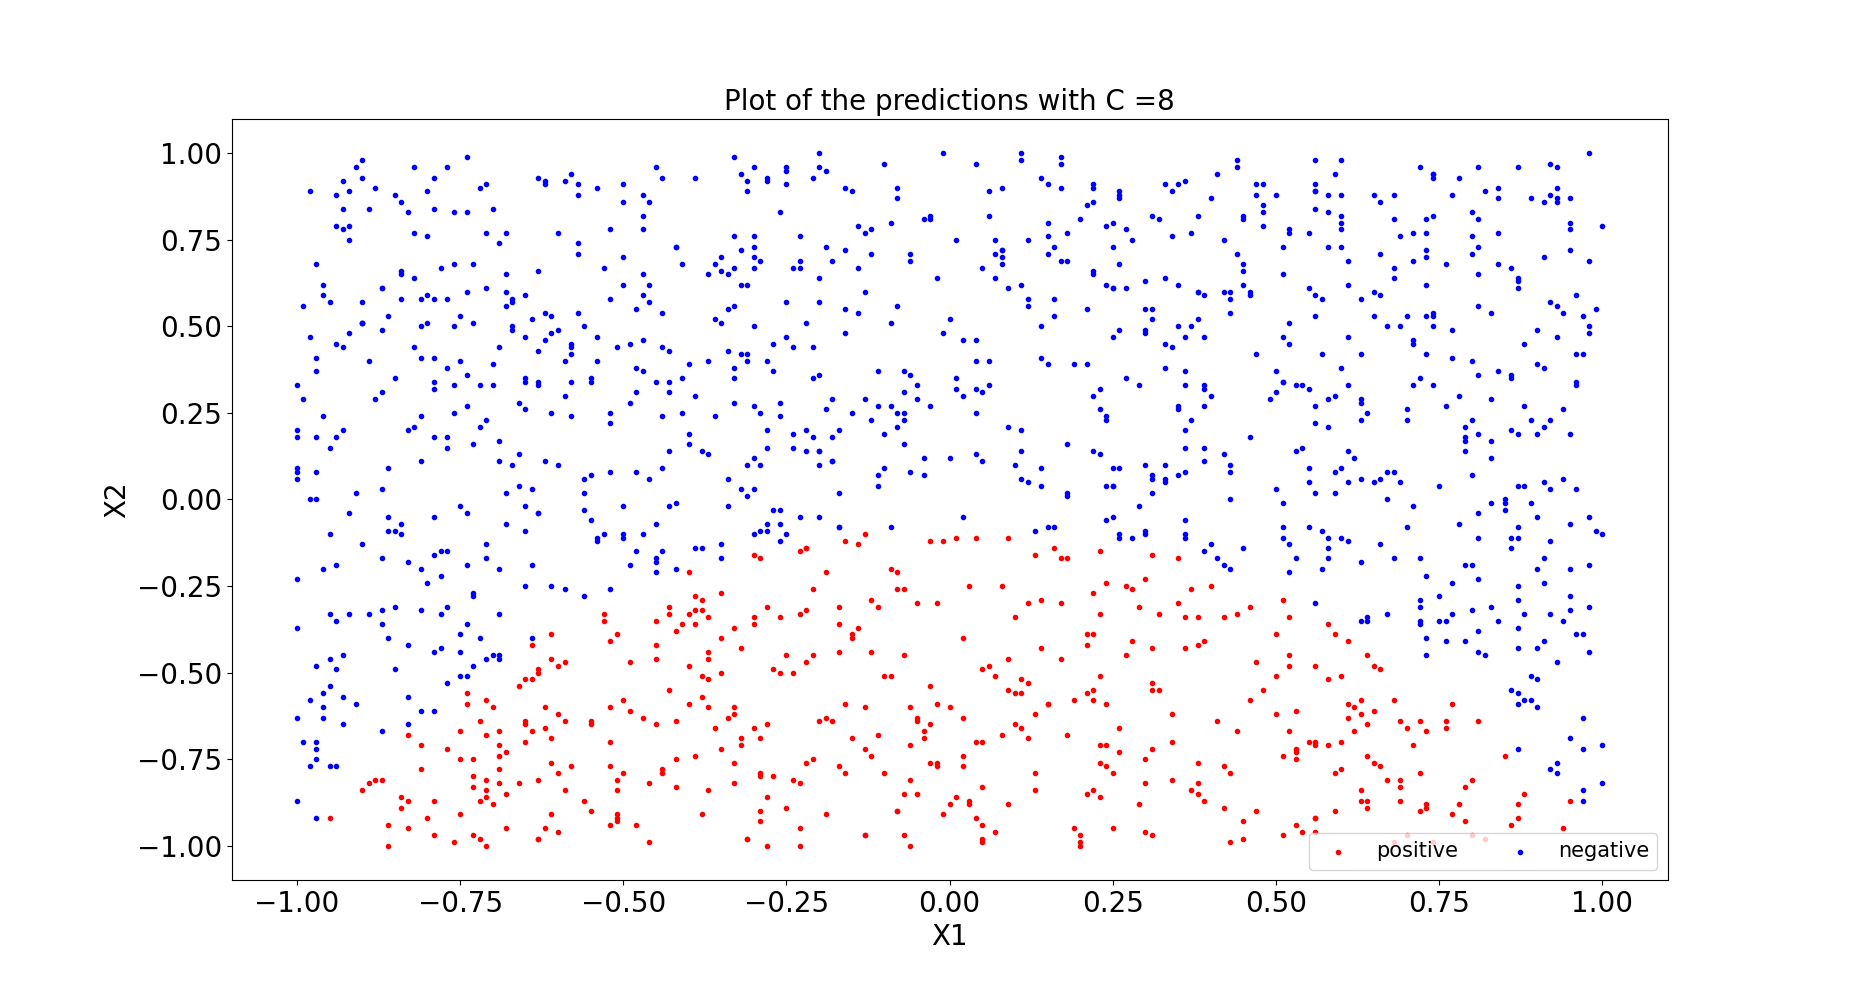
\includegraphics[scale=0.15]{ds_1_pred_c_8.png}}
    \fbox{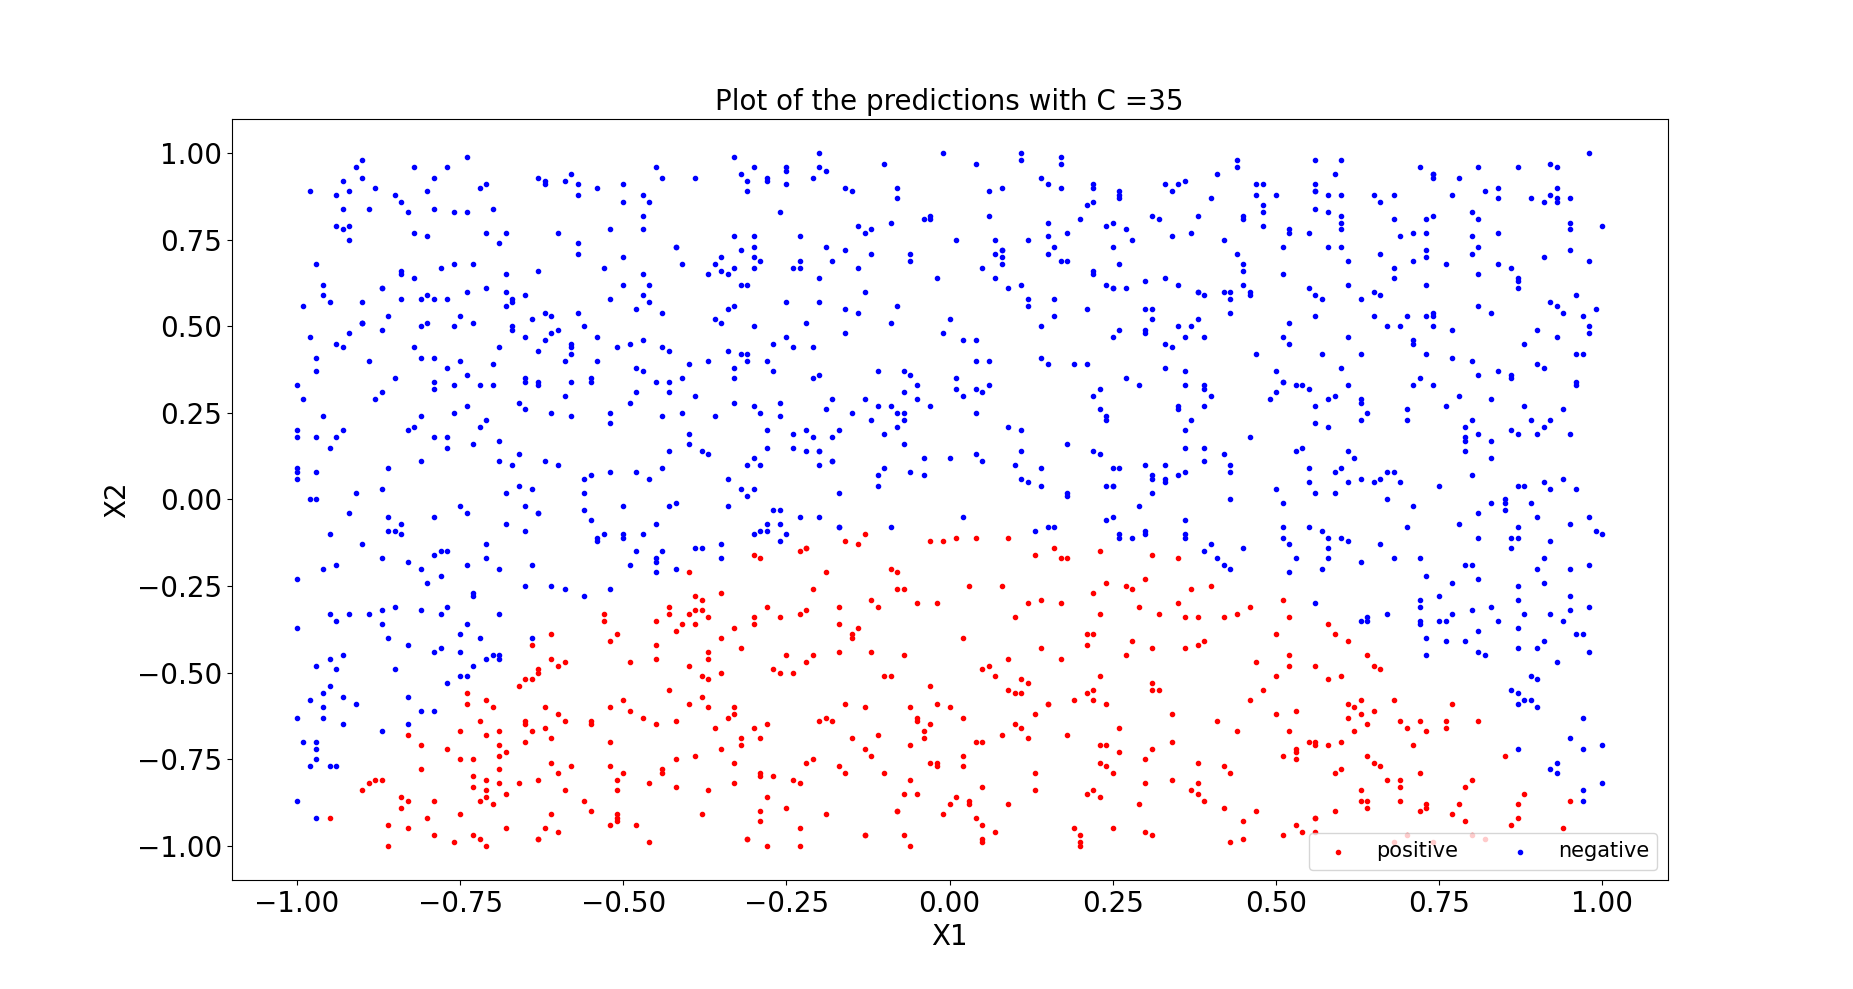
\includegraphics[scale=0.15]{ds_1_pred_c_25.png}}
\end{figure}

We notice straight away that all of the values chosen for C yeild
very similar predictions.

\subsection*{Part b}

Using sklearn's kNN model and the exact same approach as explained
previously, we can train a kNN models with a range of k values
such as to obtain a cross validation plot. Once again we also
keep track of the mean squared error such as to better inform our
decisions.

In terms of range, once again, I picked a large rage from 1 to 20,
going past 5, we clearly notice very similar results thus increasing the range
would only make computations take longer and not help our decision making.

The code for this is very similar than the one we've observed before:

\begin{lstlisting}
neighbors_range = range(1, 20, 1)
scores = []
temp = []
for n in neighbors_range:
    model = KNeighborsClassifier(
        n_neighbors=n, weights='uniform').fit(X, y)
    scores.append(model.score(X, y))
    temp.append(mean_squared_error(y, model.predict(X)))
\end{lstlisting}

We can then obtain the following cross validation plot:

\begin{center}
    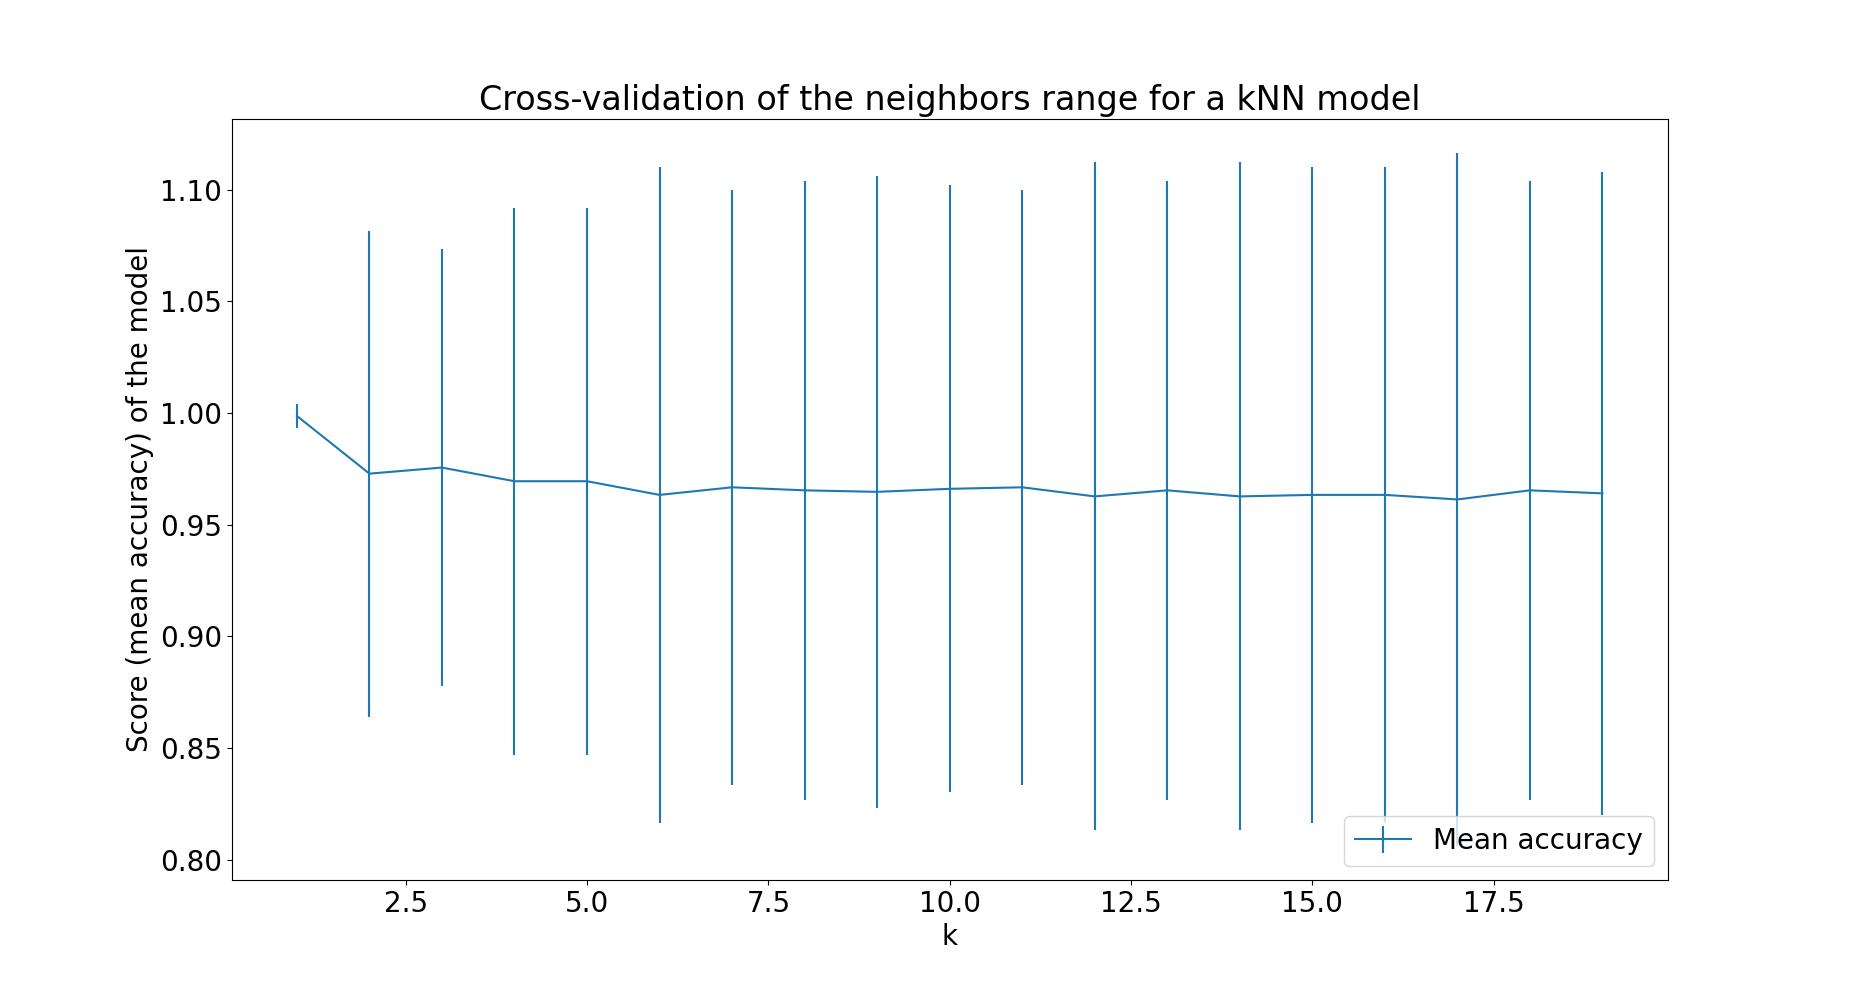
\includegraphics[scale=0.25]{ds_1_knn_cv.png}
\end{center}
\vspace{5mm} %5mm vertical space

We notice straight away that the value $ k = 1 $ is the one to pick
here as its accuracy is very close (if not) 1. The mean squared error is also clearly the lowest.

Let's plot predictions using 3 different k values to see how they compare 
against the original data:

\begin{figure}[H]    
    \fbox{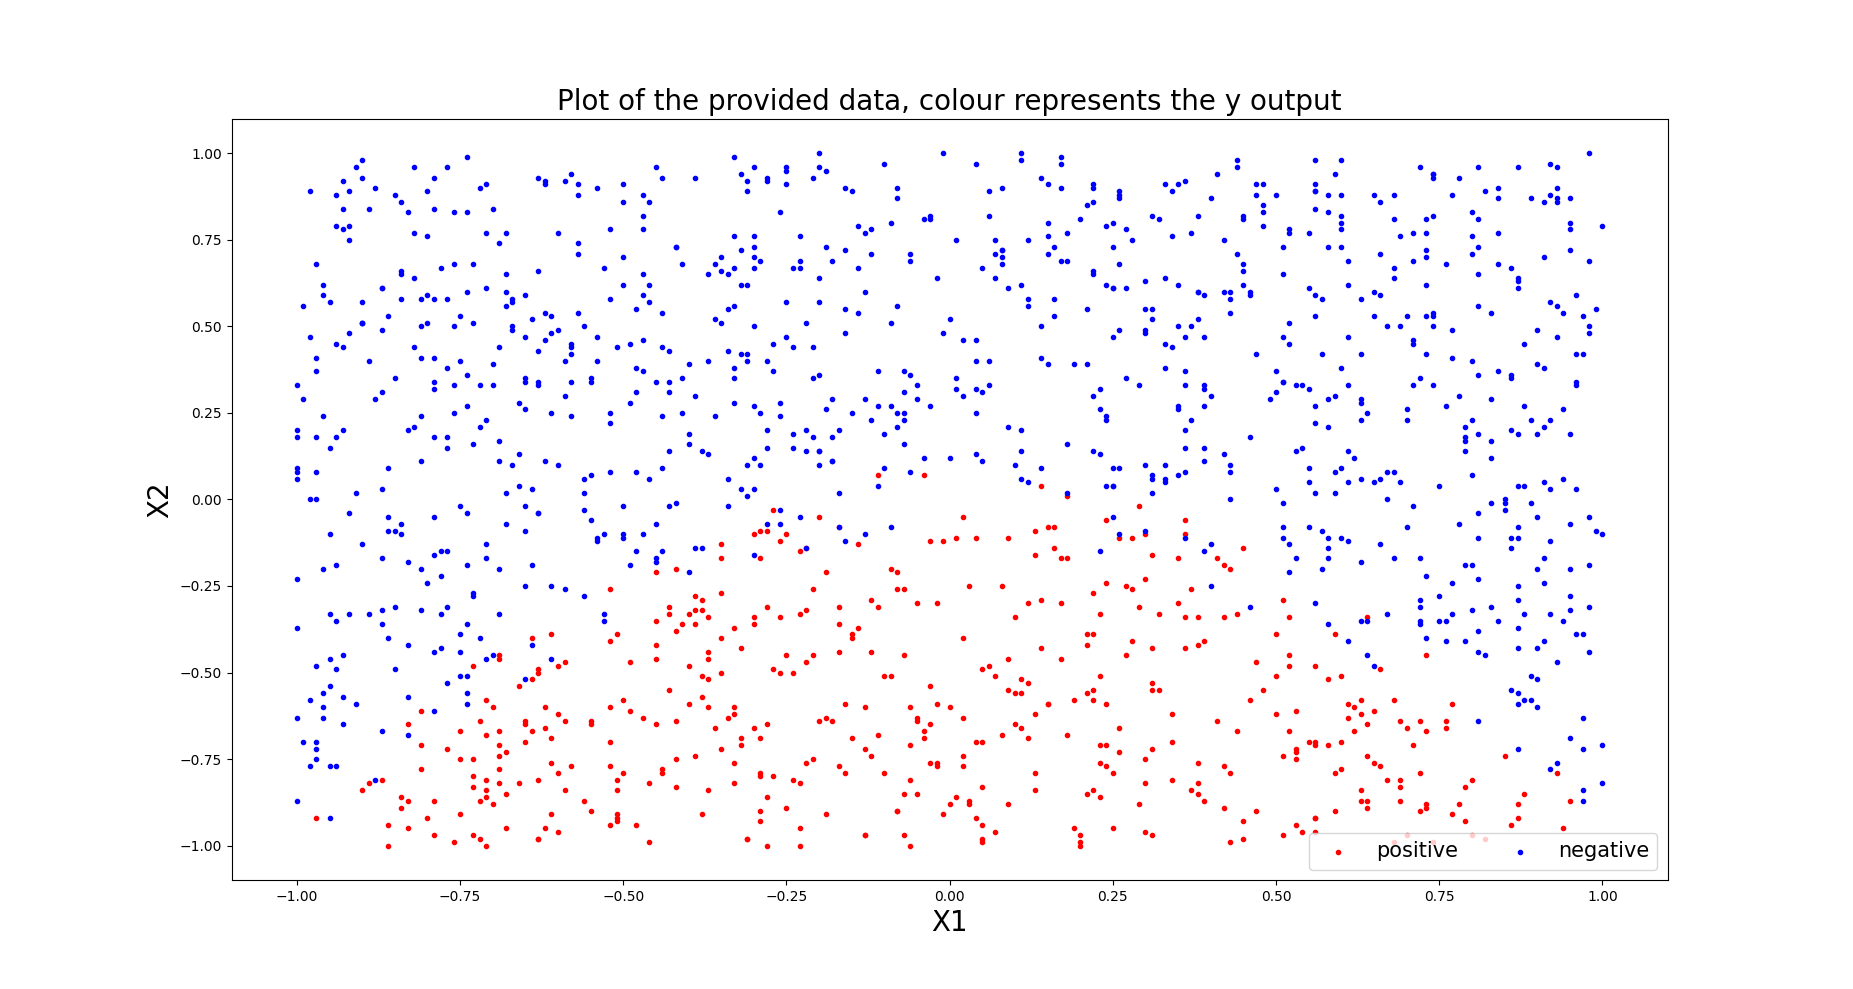
\includegraphics[scale=0.15]{Figure_1.png}}   
    \fbox{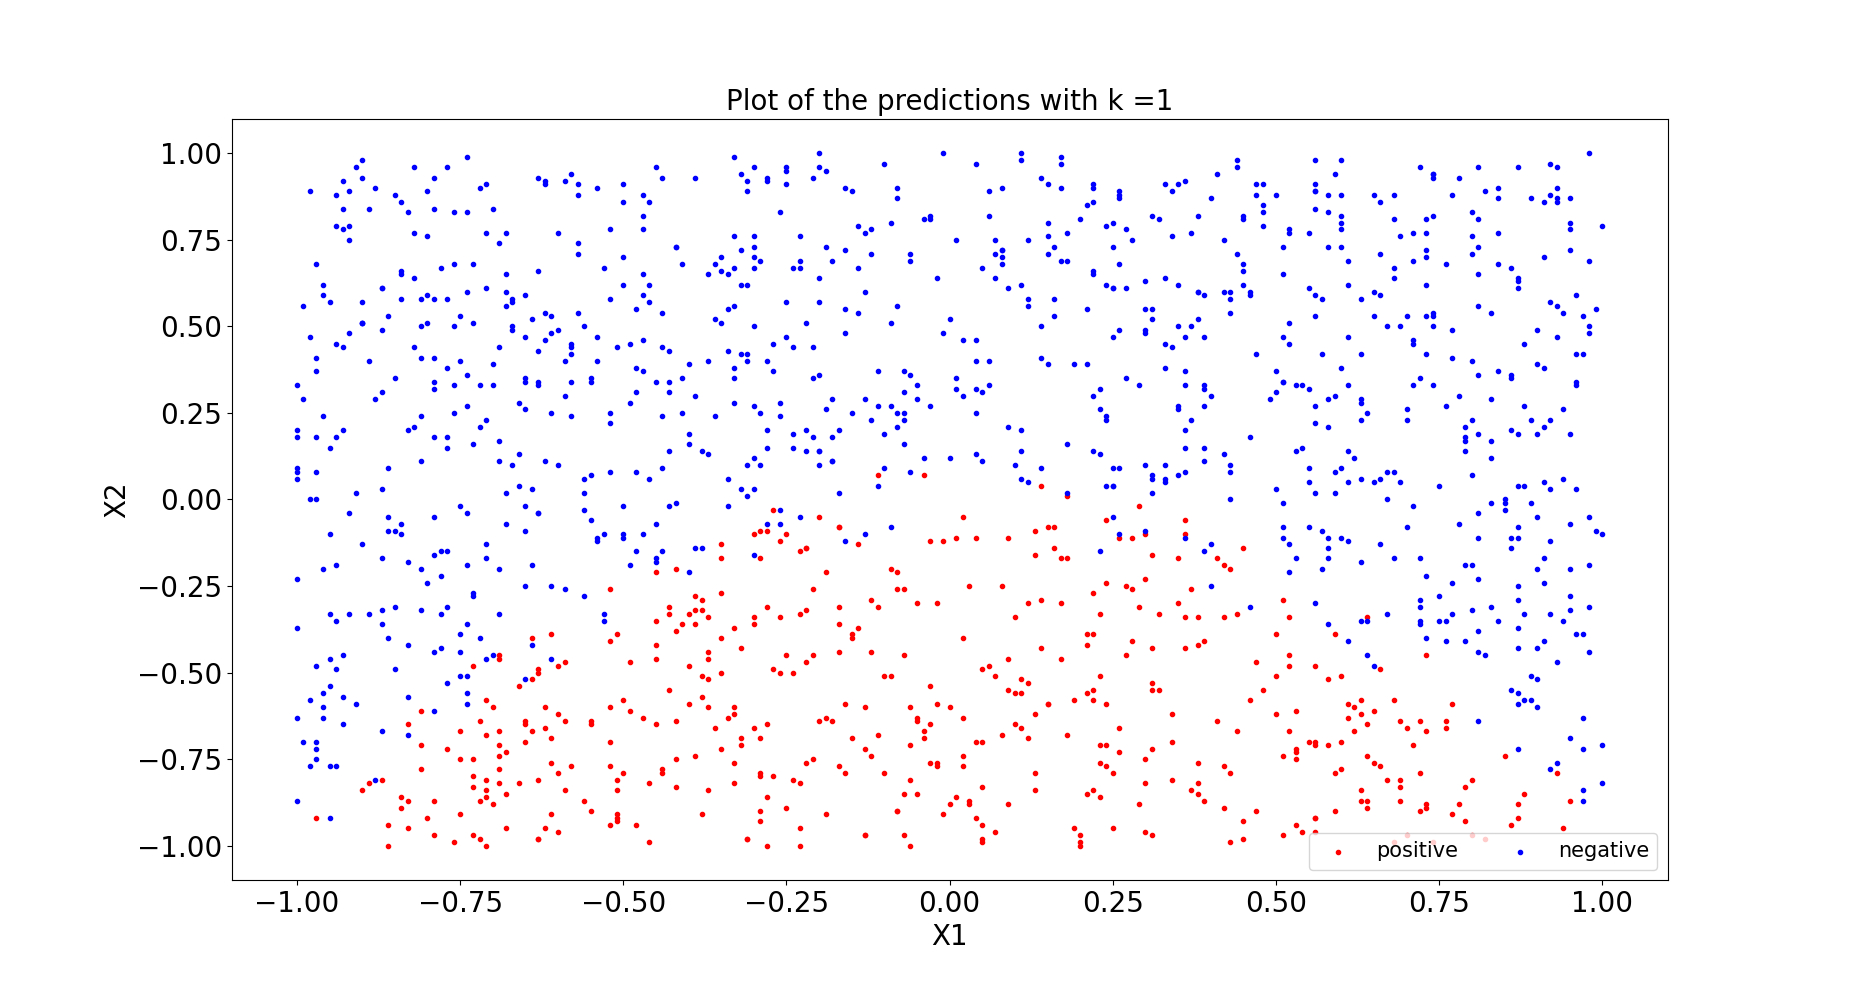
\includegraphics[scale=0.15]{ds_1_pred_knn_1.png}}   
    \fbox{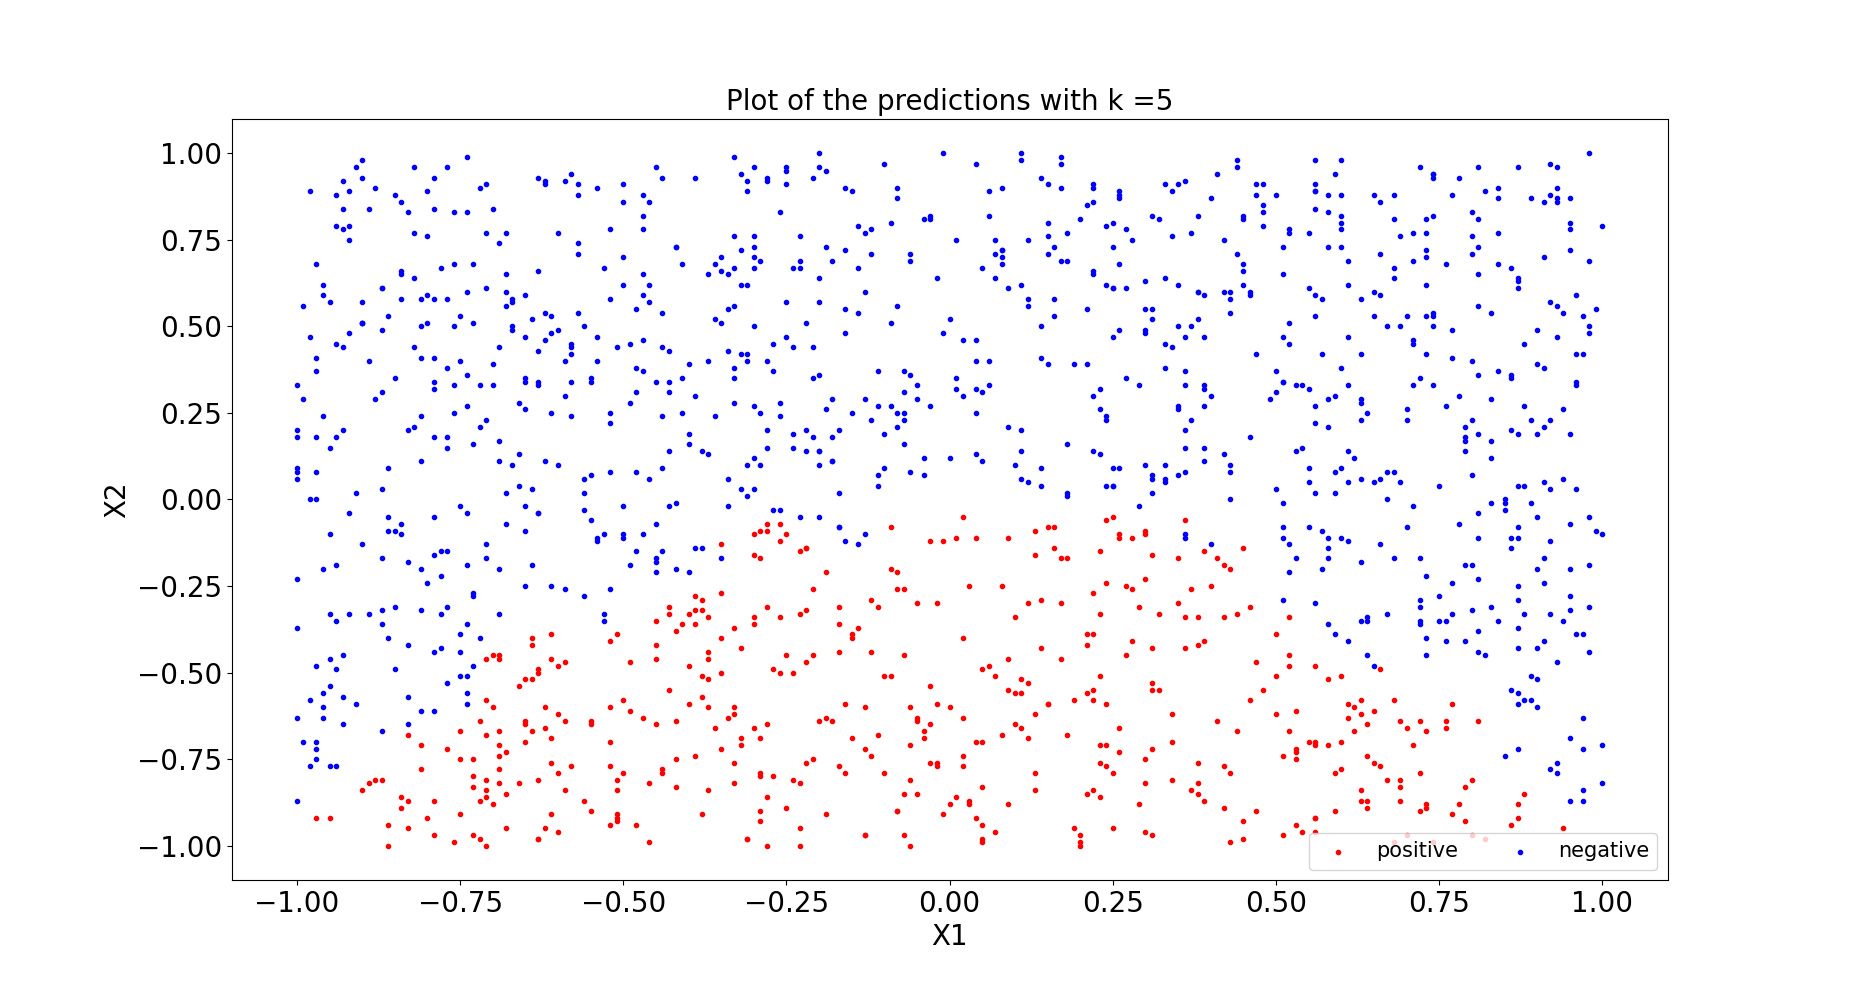
\includegraphics[scale=0.15]{ds_1_pred_knn_5.png}}
    \fbox{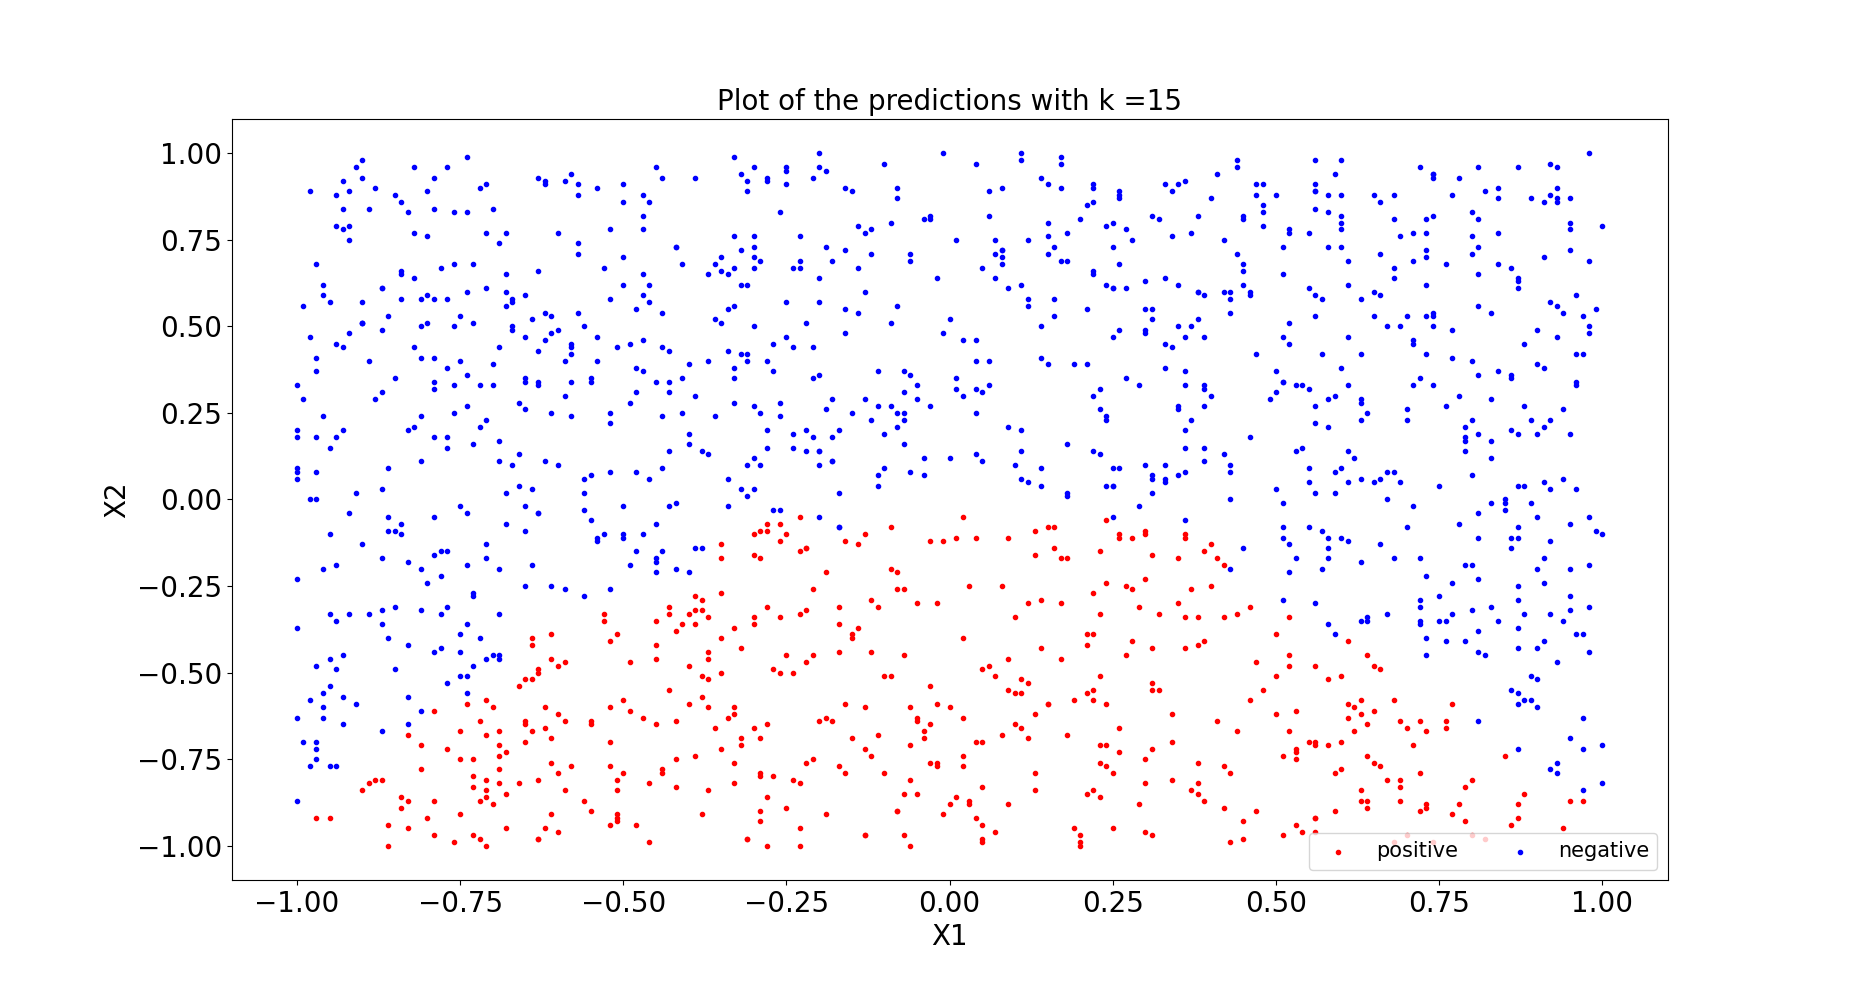
\includegraphics[scale=0.15]{ds_1_pred_knn_15.png}}
\end{figure}

We can notice that the model with $ k = 1 $ behaves better where the
the data overlaps slightly, this is due to the fact that less neighbors are
taken into account, the higher the k value the more of a clear separation we notice.

Let's now consider the possibility of potentially augmenting the feature for that kNN model.
Using the same method of cross validation for a large range of polynomial degrees, we obtain the following plot.
Note that this plot used the previously selected value $ k = 1 $.

\begin{center}
    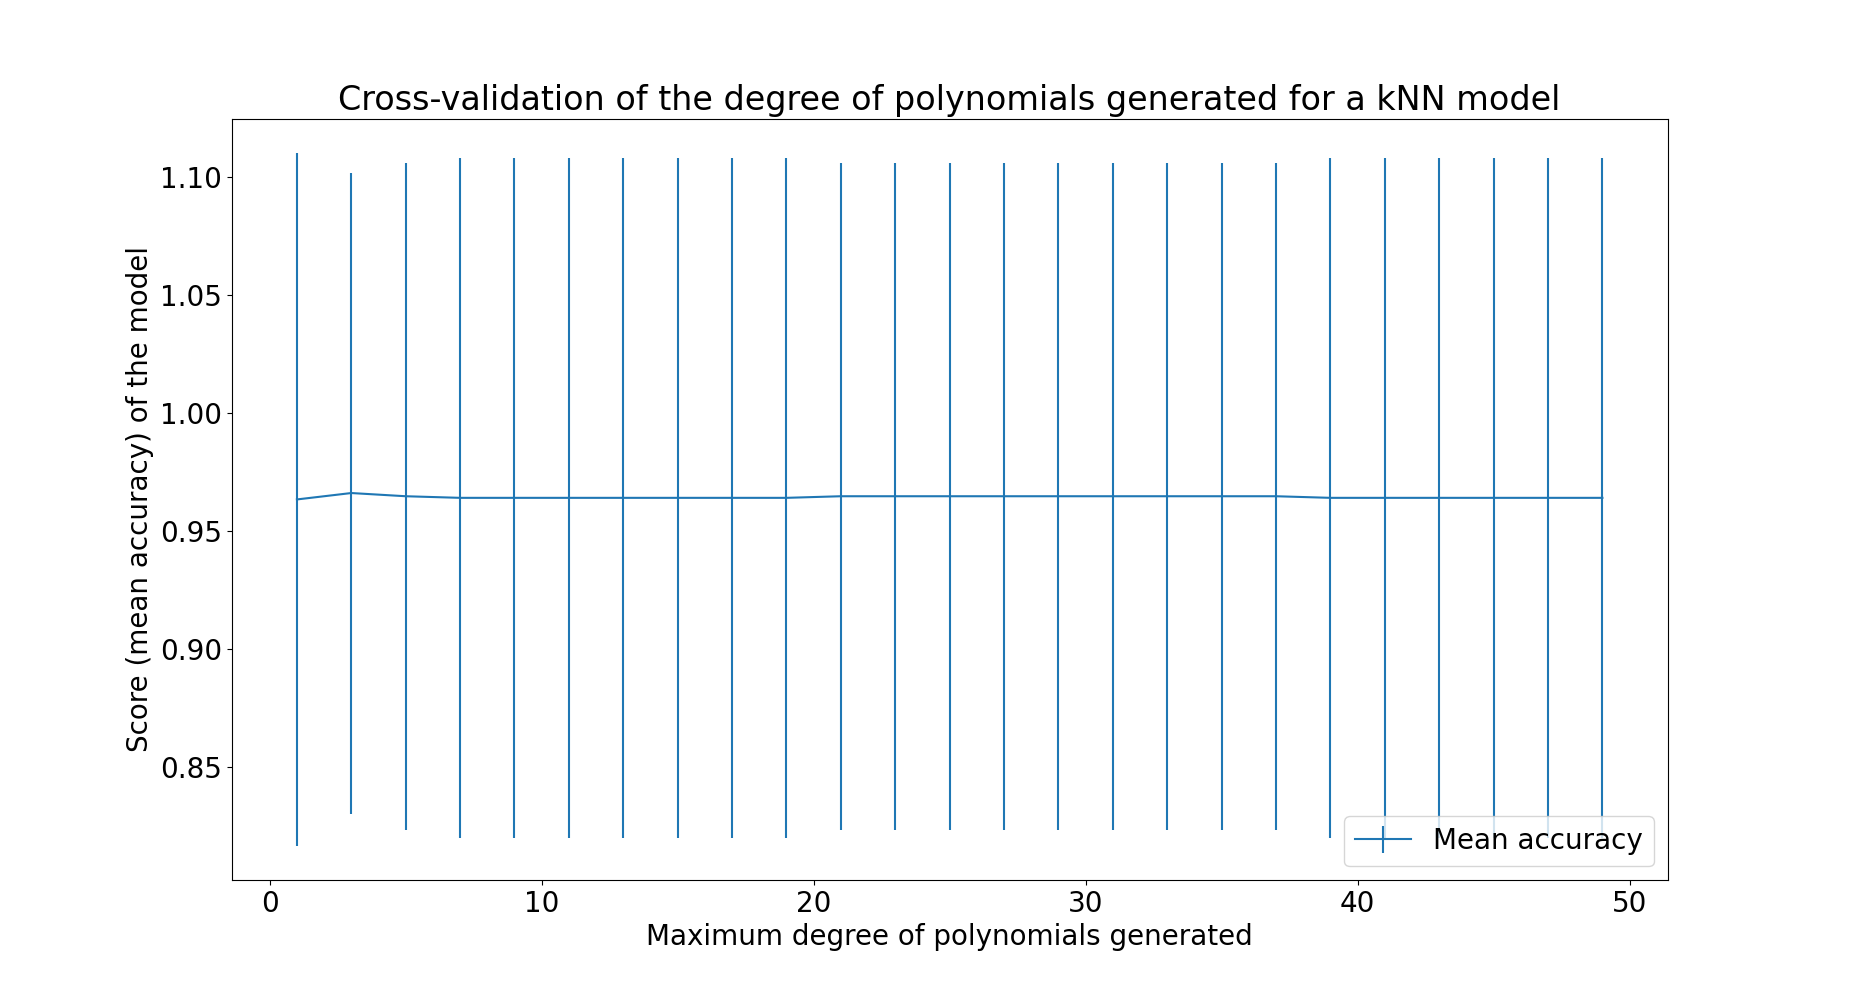
\includegraphics[scale=0.25]{ds_1_knn_d_cv.png}
\end{center}
\vspace{5mm} %5mm vertical space
We notice absolutely no advantage with our selected k value to augment the 2 features we have.
Both the accuracy and mean squared error remains roughly the same.

\subsection*{Part c}
For this part, I will train 4 models using the parameters that we identified in previous questions.
That is:
\begin{itemize}
    \item Logistic Regression (L2) model, with C = 8 and features augmented to the 2nd polynomial order.
    \item kNN Model, with k = 1 and the default provided features.
    \item Most frequent value model, a model which always predicts the most common output.
    \item Random model, a model which always predicts a random output.
  \end{itemize}


We've previously seen how to train logistic regression and kNN models, let's now address how I will
create the remaining two models. I originally had coded these by hand however it proved to be a challenge
to create ROC graphs down the line so I changed my implementation to using sklearn's DummyClassifier.

Thus implementation happens as such:

\begin{lstlisting}
randomModel = DummyClassifier(strategy="uniform")
mostFreqModel = DummyClassifier(strategy="most_frequent")

randomModel.fit(X, y)
mostFreqModel.fit(X, y)
\end{lstlisting}

Quite similar to other models, with the exception of the strategy parameter which specify which kind of
baseline model to use.

I can then obtain the confusion matrix using the $confusion\_matrix$ method from sklearn,
we give it as input the actual y outputs and the predictions for a specific model.
\begin{lstlisting}
knn_pred = knnModel.predict(X)
tn, fp, fn, tp = confusion_matrix(y, knn_pred).ravel()
\end{lstlisting}

Doing this for all 4 models, and putting the outputs in a table, we obtain the following:
\par
\vspace{5mm} %5mm vertical space
ROC Table for the kNN model, using k = 1 and the default features from the dataset:
\par
\vspace{5mm} %5mm vertical space
\begin{tabularx}{0.8\textwidth} { 
    | >{\raggedright\arraybackslash}X 
    | >{\centering\arraybackslash}X 
    | >{\raggedleft\arraybackslash}X | }
    \hline
     & Predicted positive & Predicted negative \\
    \hline
    True positive & 989 & 2 \\
   \hline
   True negative  & 0 & 480 \\
  \hline
\end{tabularx}
\par
We notice straight away that the predictions are close to perfect, with only 2 predictions
not being correct.
\par
\vspace{5mm} %5mm vertical space
ROC Table for the Logistic Regression model, using $ C = 8 $ and
transforming the features using PolynomialFeatures up to a degree of 2.
\par
\vspace{5mm} %5mm vertical space
\begin{tabularx}{0.8\textwidth} { 
    | >{\raggedright\arraybackslash}X 
    | >{\centering\arraybackslash}X 
    | >{\raggedleft\arraybackslash}X | }
    \hline
     & Predicted positive & Predicted negative \\
    \hline
    True positive & 967 & 24 \\
   \hline
   True negative  & 29 & 451 \\
  \hline
\end{tabularx}
\par
We notice that predictions here are quite good, with the vast majority
of predictions being correct, however we find that 53 predictions were false
which is much higher than that of the kNN model.
\par
\vspace{5mm} %5mm vertical space
ROC Table for the Random model:
\par
\vspace{5mm} %5mm vertical space
\begin{tabularx}{0.8\textwidth} { 
    | >{\raggedright\arraybackslash}X 
    | >{\centering\arraybackslash}X 
    | >{\raggedleft\arraybackslash}X | }
    \hline
     & Predicted positive & Predicted negative \\
    \hline
    True positive & 483 & 508 \\
   \hline
   True negative  & 230 & 250 \\
  \hline
\end{tabularx}
\par
Here we notice that the values are a bit all over the place, this makes sense as our model
is truly random thus it is expected.
\par
\vspace{5mm} %5mm vertical space
ROC Table for the Most frequent value model:
\par
\vspace{5mm} %5mm vertical space
\begin{tabularx}{0.8\textwidth} { 
    | >{\raggedright\arraybackslash}X 
    | >{\centering\arraybackslash}X 
    | >{\raggedleft\arraybackslash}X | }
    \hline
     & Predicted positive & Predicted negative \\
    \hline
    True positive & 991 & 0 \\
   \hline
   True negative  & 480 & 0 \\
  \hline
\end{tabularx}
\par
For this final model we only find true positives and true negatives,
this makes sense as our model predicts the most common value (which in this case is
positive). We find that roughly 2/3rds of predictions are correct.

\subsection*{Part d}
For this section, we use the same models as discussed in the previous question.
In order to plot the ROC curves, I used the $roc\_curve$ method from sklearn.
That method can take either the decision function from the model or the probability
estimates for the positive class. Sklearn models sometimes have one or the other so
I had to use a mix of both methods here:

\begin{lstlisting}
# logistic roc
fpr, tpr, _ = roc_curve(y,
        lgModel.decision_function(X_poly))
# knn roc
knn_proba = knnModel.predict_proba(X)
knn_fpr, knn_tpr, thresh = roc_curve(y, knn_proba[:, 1])
\end{lstlisting}
\par
The plotting itself is quite straightfoward from here, it consists of simple
line plots using both outputs from the roc function:
\par
\begin{lstlisting}
ax.plot(fpr, tpr, color='cyan')
ax.plot(knn_fpr, knn_tpr, color='orange')
ax.plot(most_freq_fpr, most_freq_tpr, color='blue')
ax.plot(rand_fpr, rand_tpr, color='red')
ax.plot([0, 1], [0, 1], color='green', linestyle='--')
\end{lstlisting}
We then obtain the following plots:
\begin{center}
    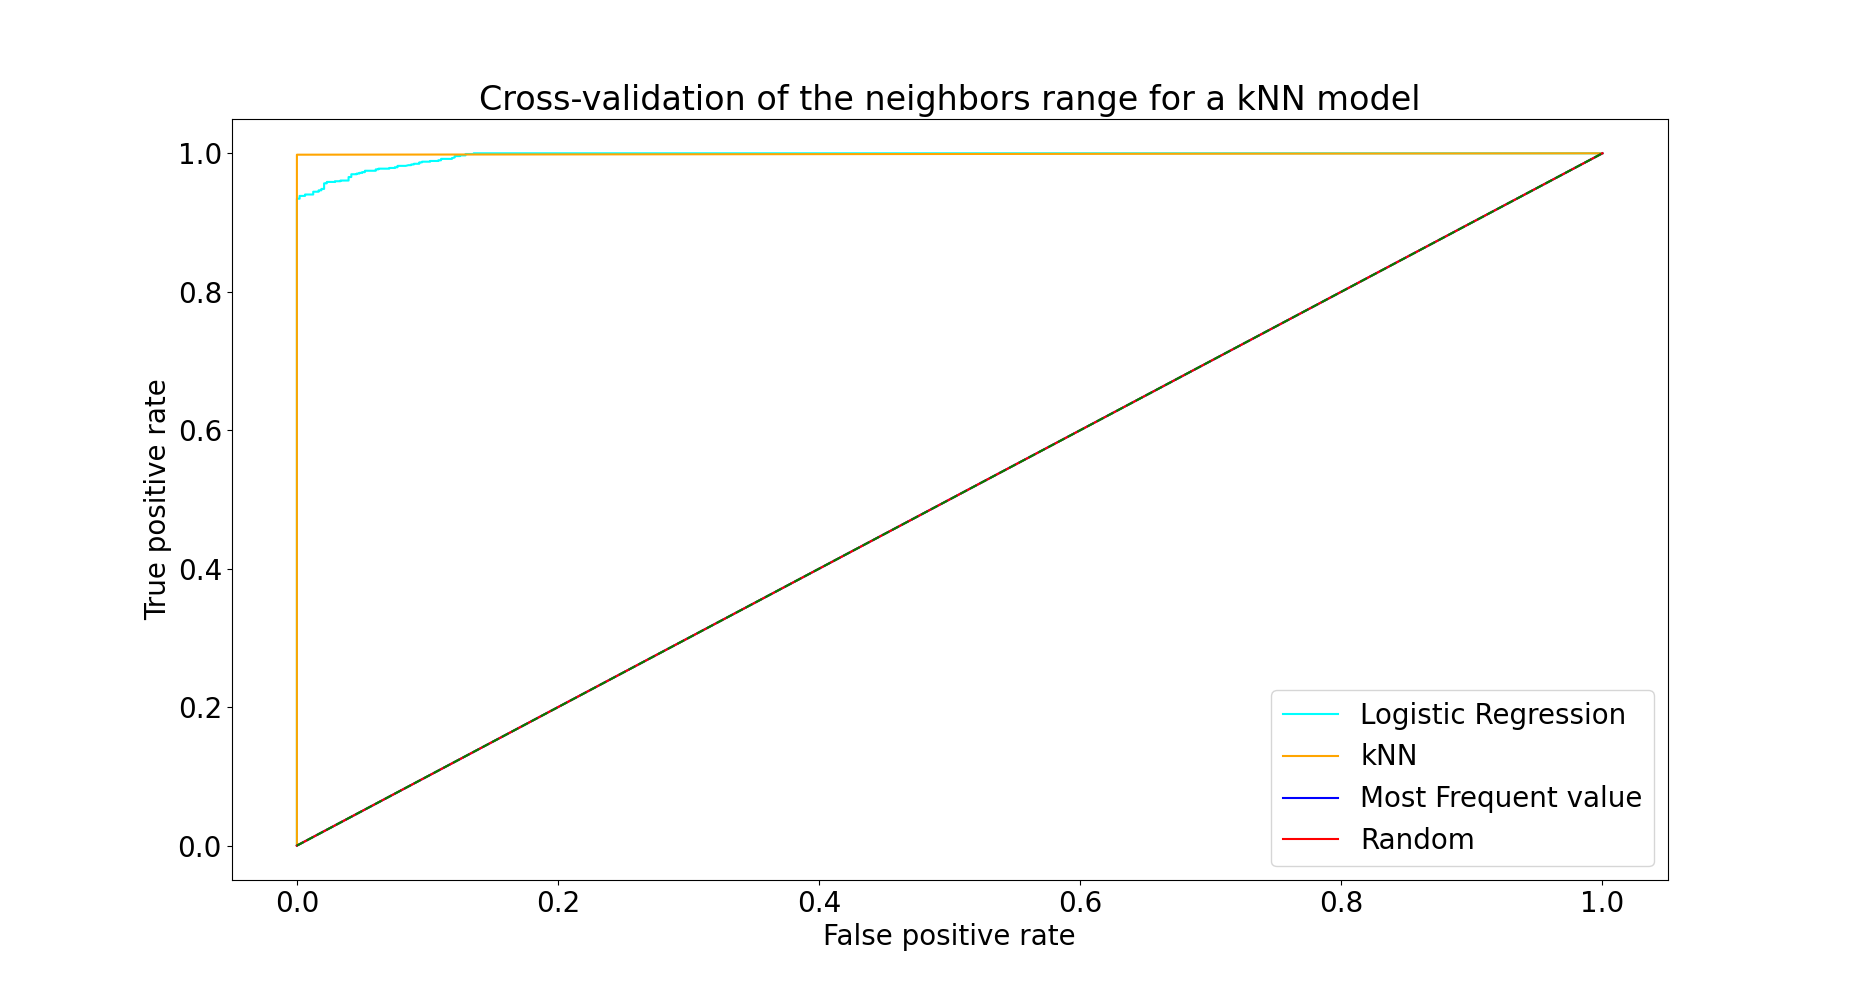
\includegraphics[scale=0.25]{roc.png}
\end{center}
\vspace{5mm} %5mm vertical space

We can clearly see that both the Logistic and kNN models are doing quite well, especially the kNN.
As expected, the random and most frequent value models are just a simple line going through the
center of the plot.

\subsection*{Part e}
Let's start with the random model, we can clearly see that its confusion matrix is by far
the worst out of all of our models, that is because the outputs are compeletely unpredictable so let's move on.
\par
Our second baseline model is the most frequent value baseline model. We find that in this case it behaves
much better than our random model, getting roughly 2/3rds of predictions right. However we find that this advantage
doesn't quite translate with the ROC curve unfortunately.
\par
Let's now consider our more sophisticated models, the logistic regression model and the kNN.
The first thing we notice on the ROC curve is that they are very high and thus predictions for both of these models
will be very accurate.
Most notably, with notice that the kNN model only predicted 2 values which weren't valid, this is quite impressive, we
can also notice this on its ROC curve, being always 1 on the true positive axis no matter the false positive rate.
Finally, to comment a bit more on the logistic model, its predictions are still very good, with its ROC curve only slightly
dropping and false negative / positives summing to about 54. It is still quite a good model for predictions however it is not
as accurate as the kNN model.
\par
To conclude, the kNN model is the clear winner here. On top of that it does not require to re-compute features thus saving
some computing power.


\section*{Question ii}
The code is the exact same as for question i thus in this section I will not be re-explaining
how I obtained some plots or trained the models, but instead focus on justifying my choices.
\subsection*{Part a}
Using the second dataset, I plotted the cross validation for selection of
polynomial order value, using any large range of degrees here we notice that clearly the system does not
benefit at all for augmenting the set of features provided for a logistic regression model.

\begin{center}
    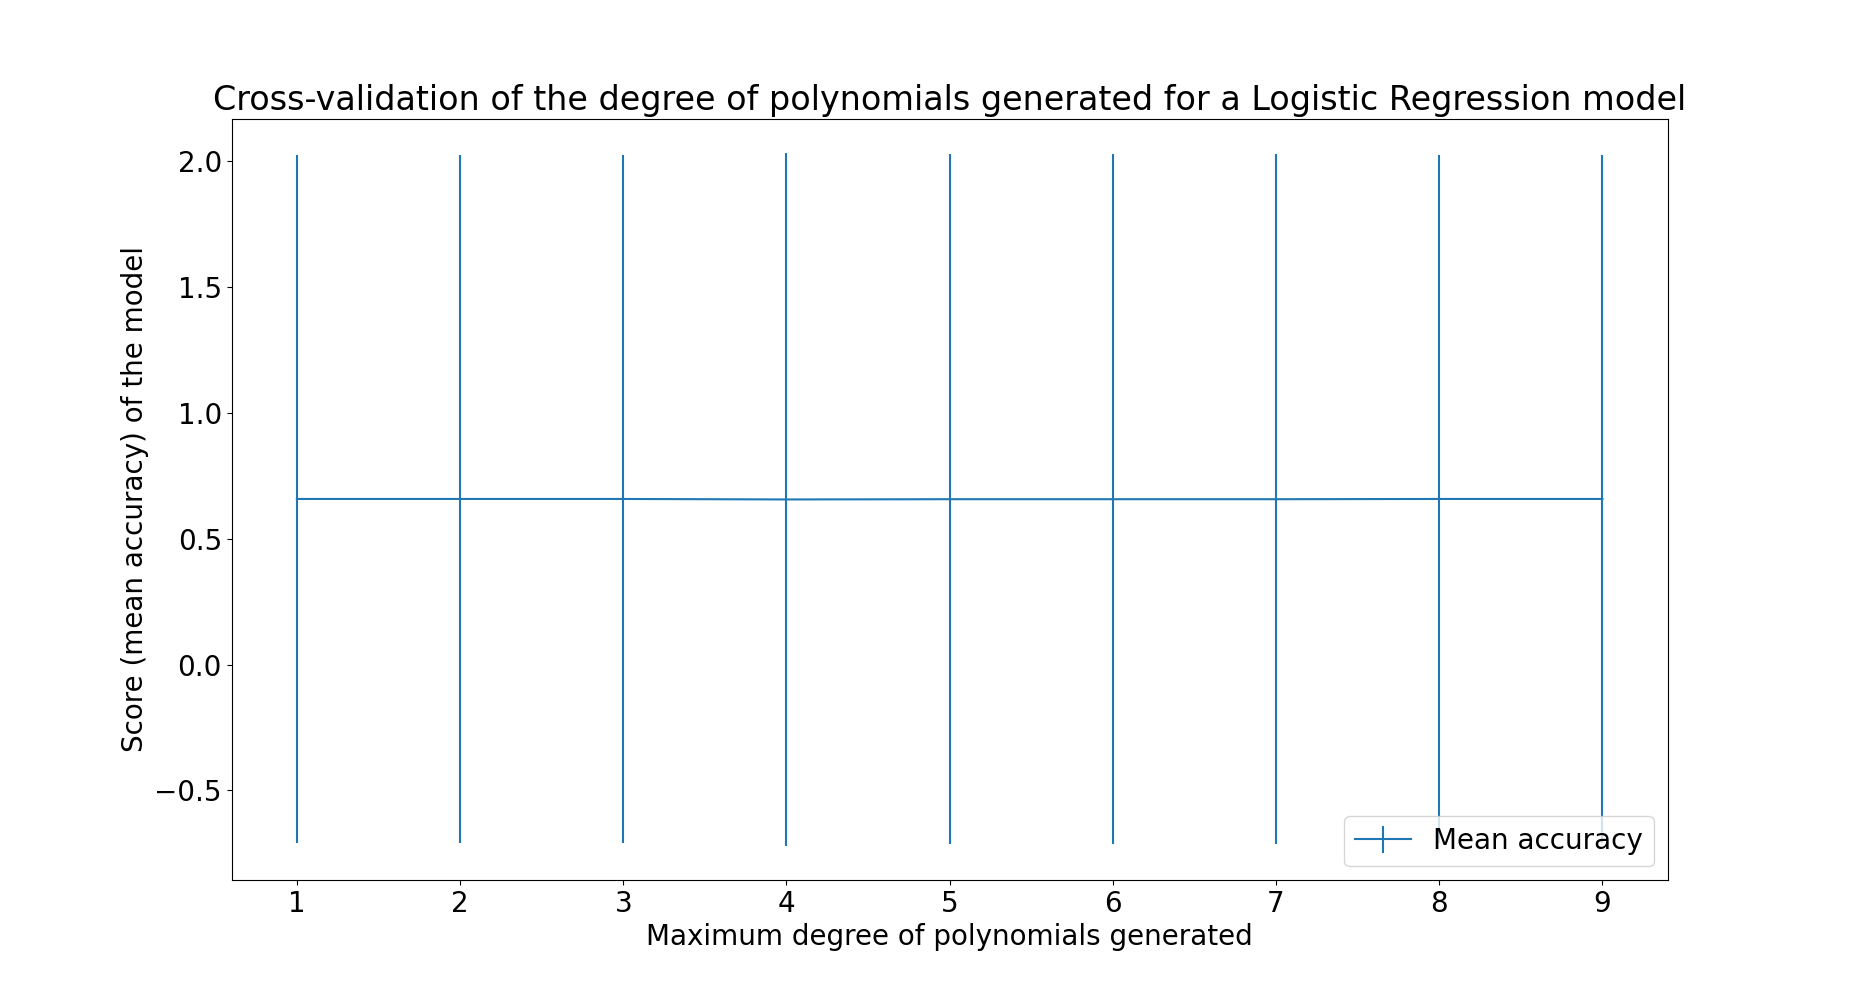
\includegraphics[scale=0.25]{ds_2_degree_cv.png}
\end{center}
\vspace{5mm} %5mm vertical space

Let's compare predictions we obtain with such a model (as we've just seen any degree of polynomial yeilds
the same score) against the actual values of the dataset:

\begin{figure}[H]    
    \fbox{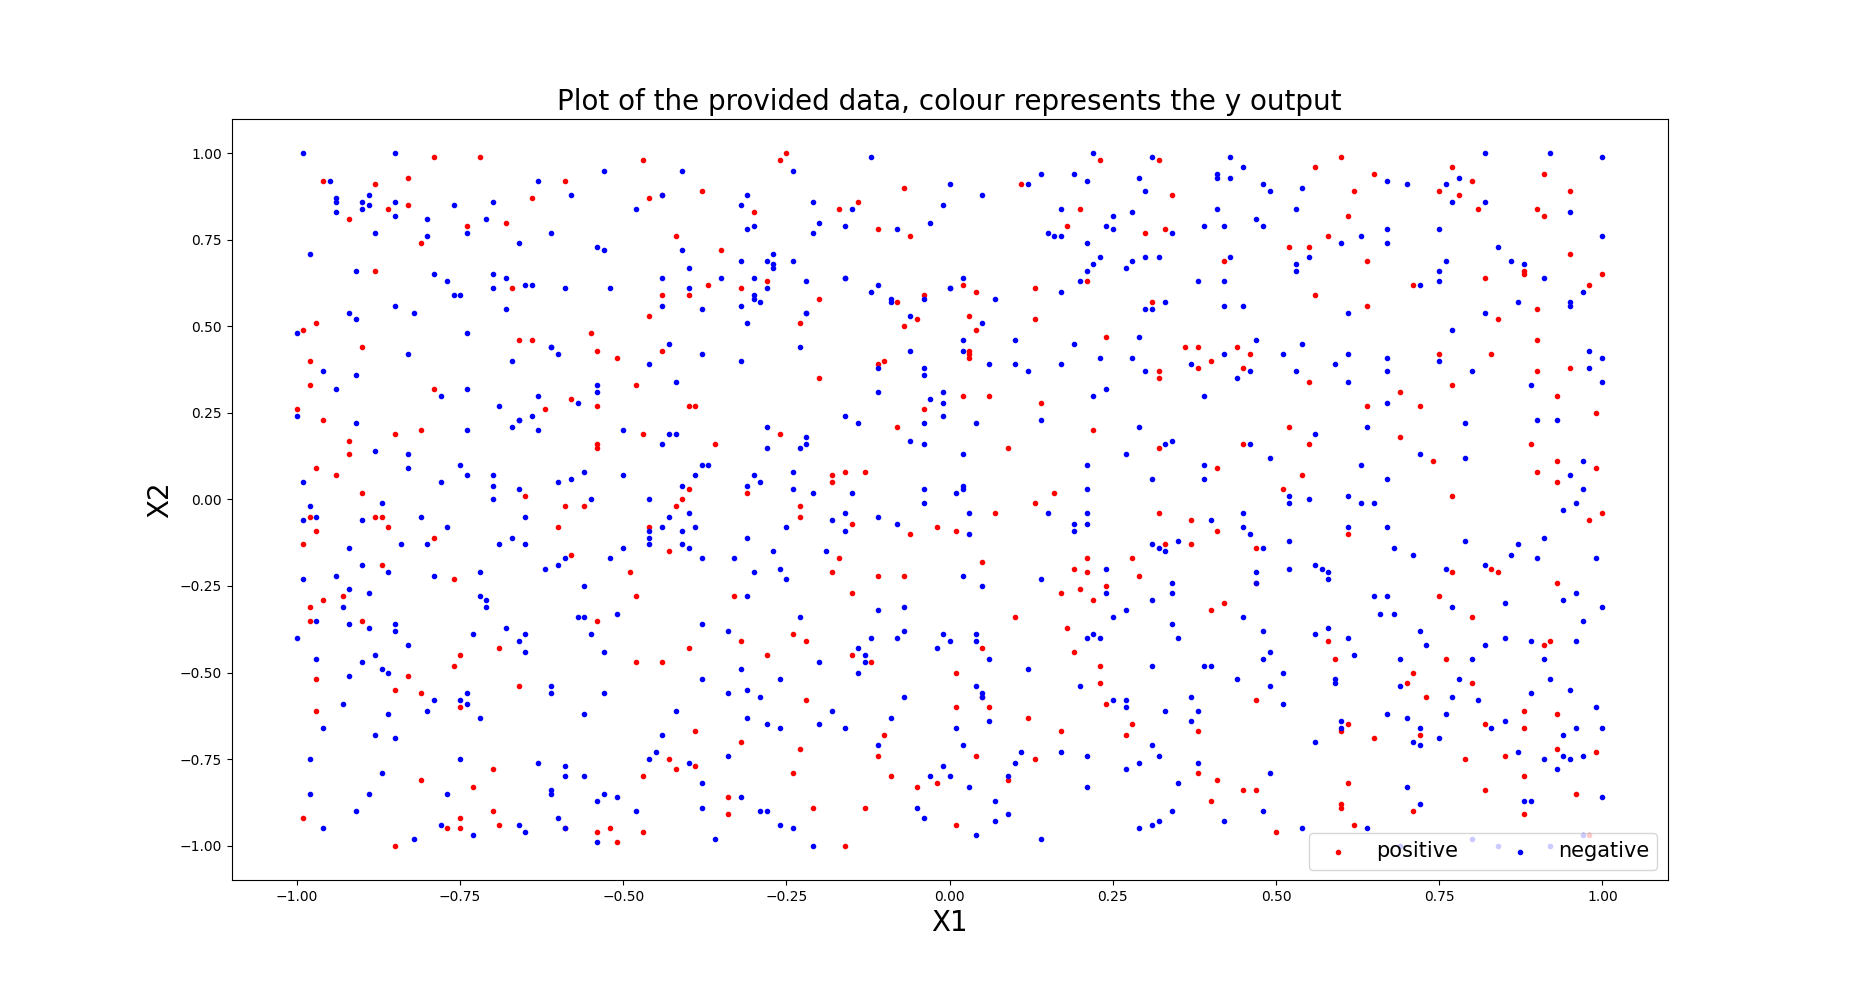
\includegraphics[scale=0.2]{Figure_2.png}}   
    \fbox{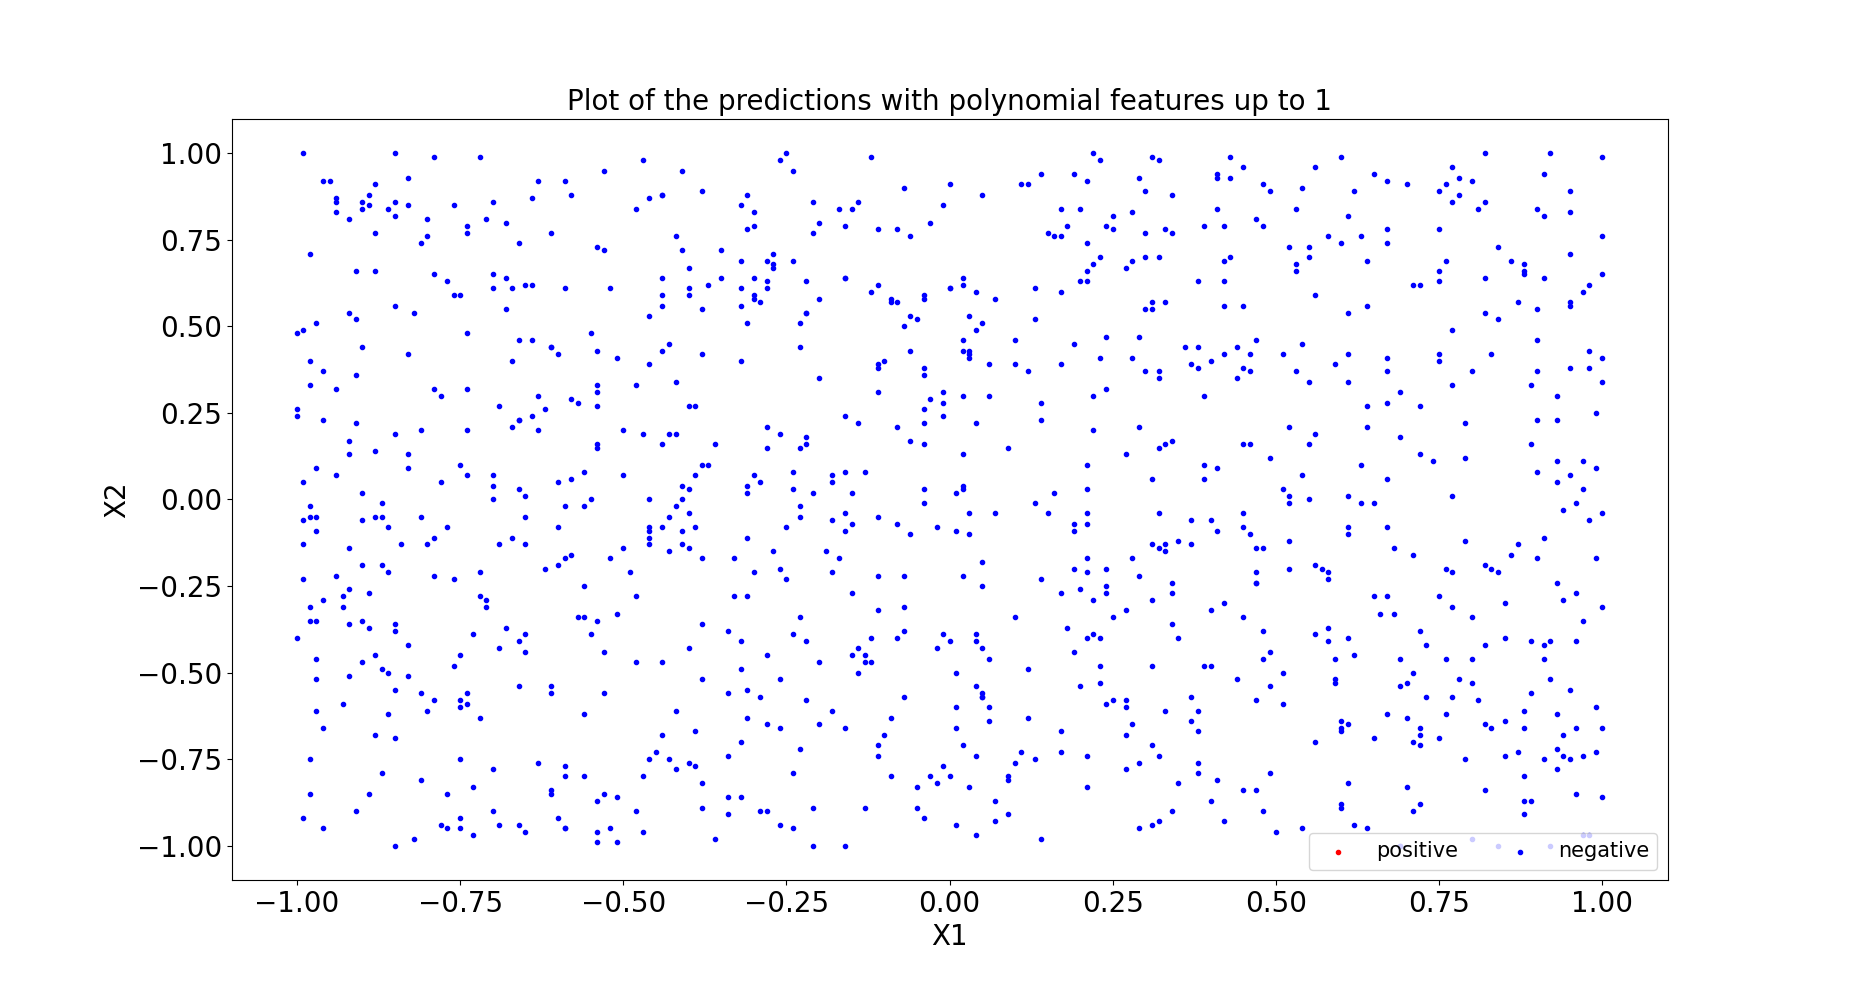
\includegraphics[scale=0.2]{ds_2_pred_d_1.png}}   
\end{figure}

We can clearly see that the data as it is is not linearly seperable and that our predictions
simply pick the most frequent output.

\vspace{5mm} %5mm vertical space

Given that varying the parameter C does not change our model here I will not plot our models
predictions here as they will be the exact same as we've already seen above.

\subsection*{Part b}

Training a kNN models with a range of k values such as to obtain a cross validation plot, using
a large range of values such that we are confident that variations of model scores worth noting
are within our range, we obtain the following cross validation plot:

\begin{center}
    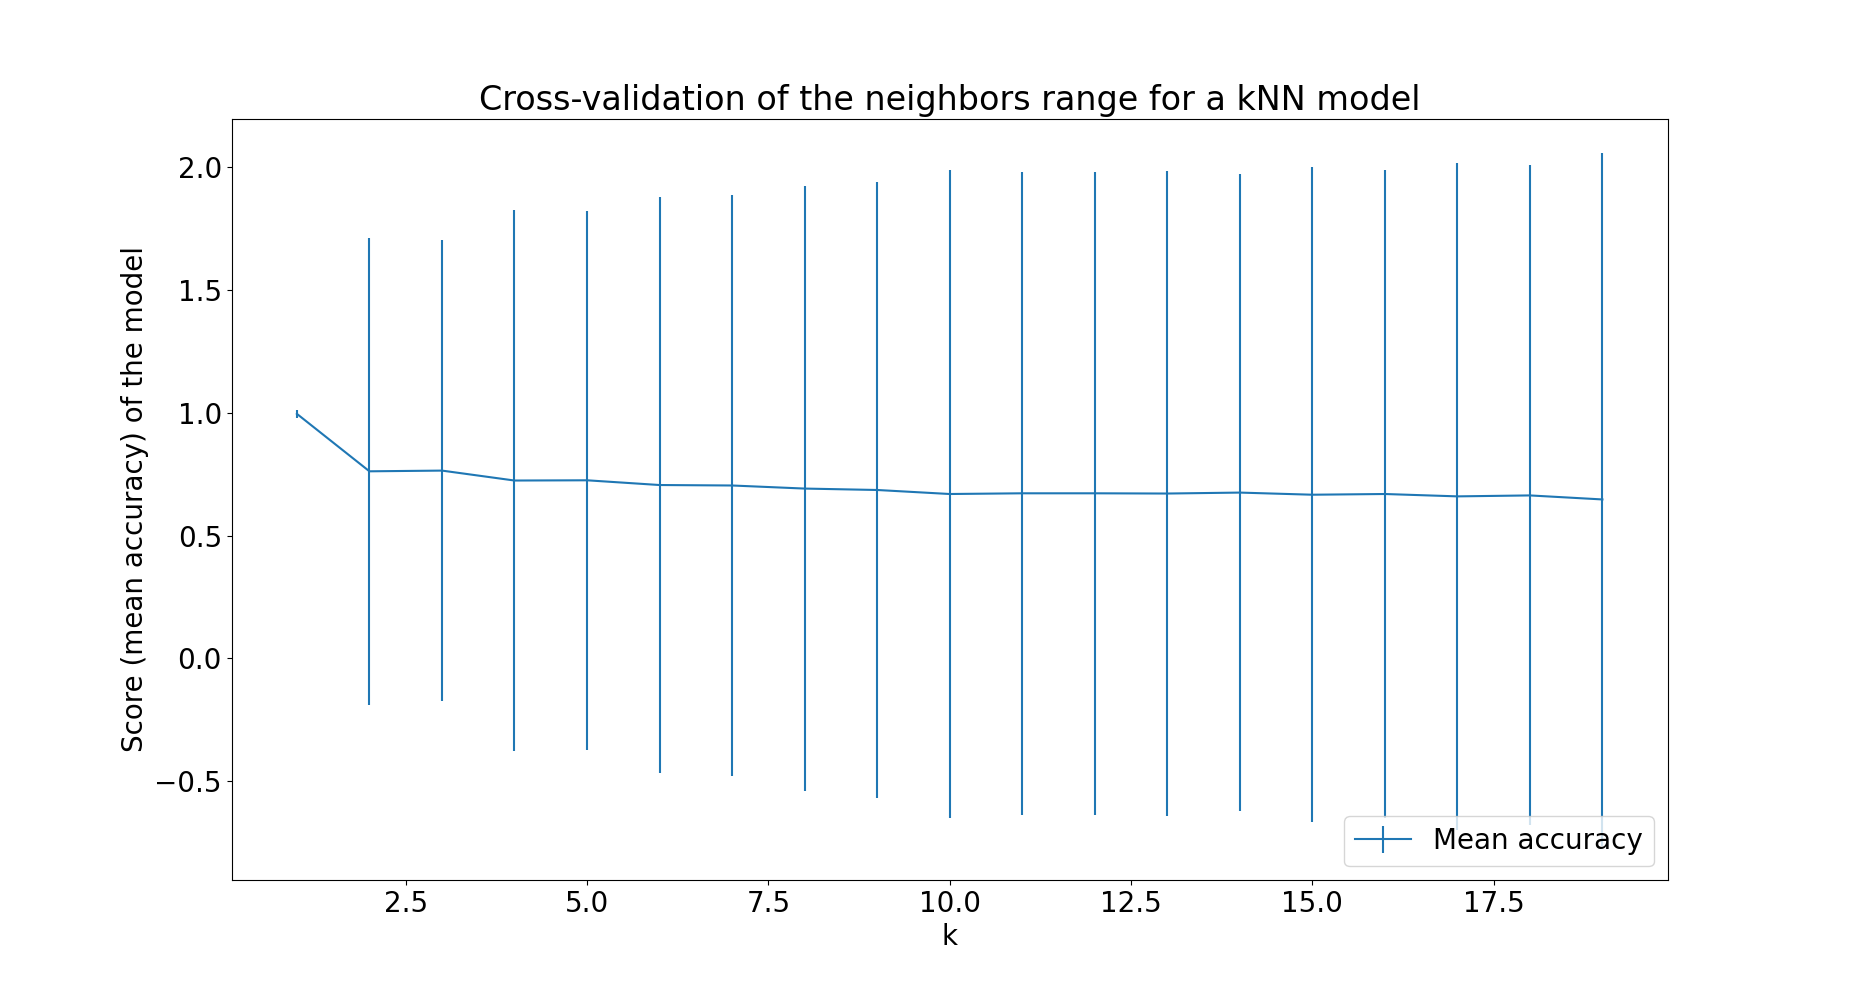
\includegraphics[scale=0.25]{ds_2_knn_cv.png}
\end{center}
\vspace{5mm} %5mm vertical space

We notice straight away that the value $ k = 1 $ is the one to pick
here as its accuracy is very close (if not) 1. The mean squared error is also clearly the lowest.
Then, as the value of k increases, it seems that so does the mean squared error and the model score
decreases. 
\par
Let's plot predictions using 3 different k values to see how they compare 
against the original data:

\begin{figure}[H]    
    \fbox{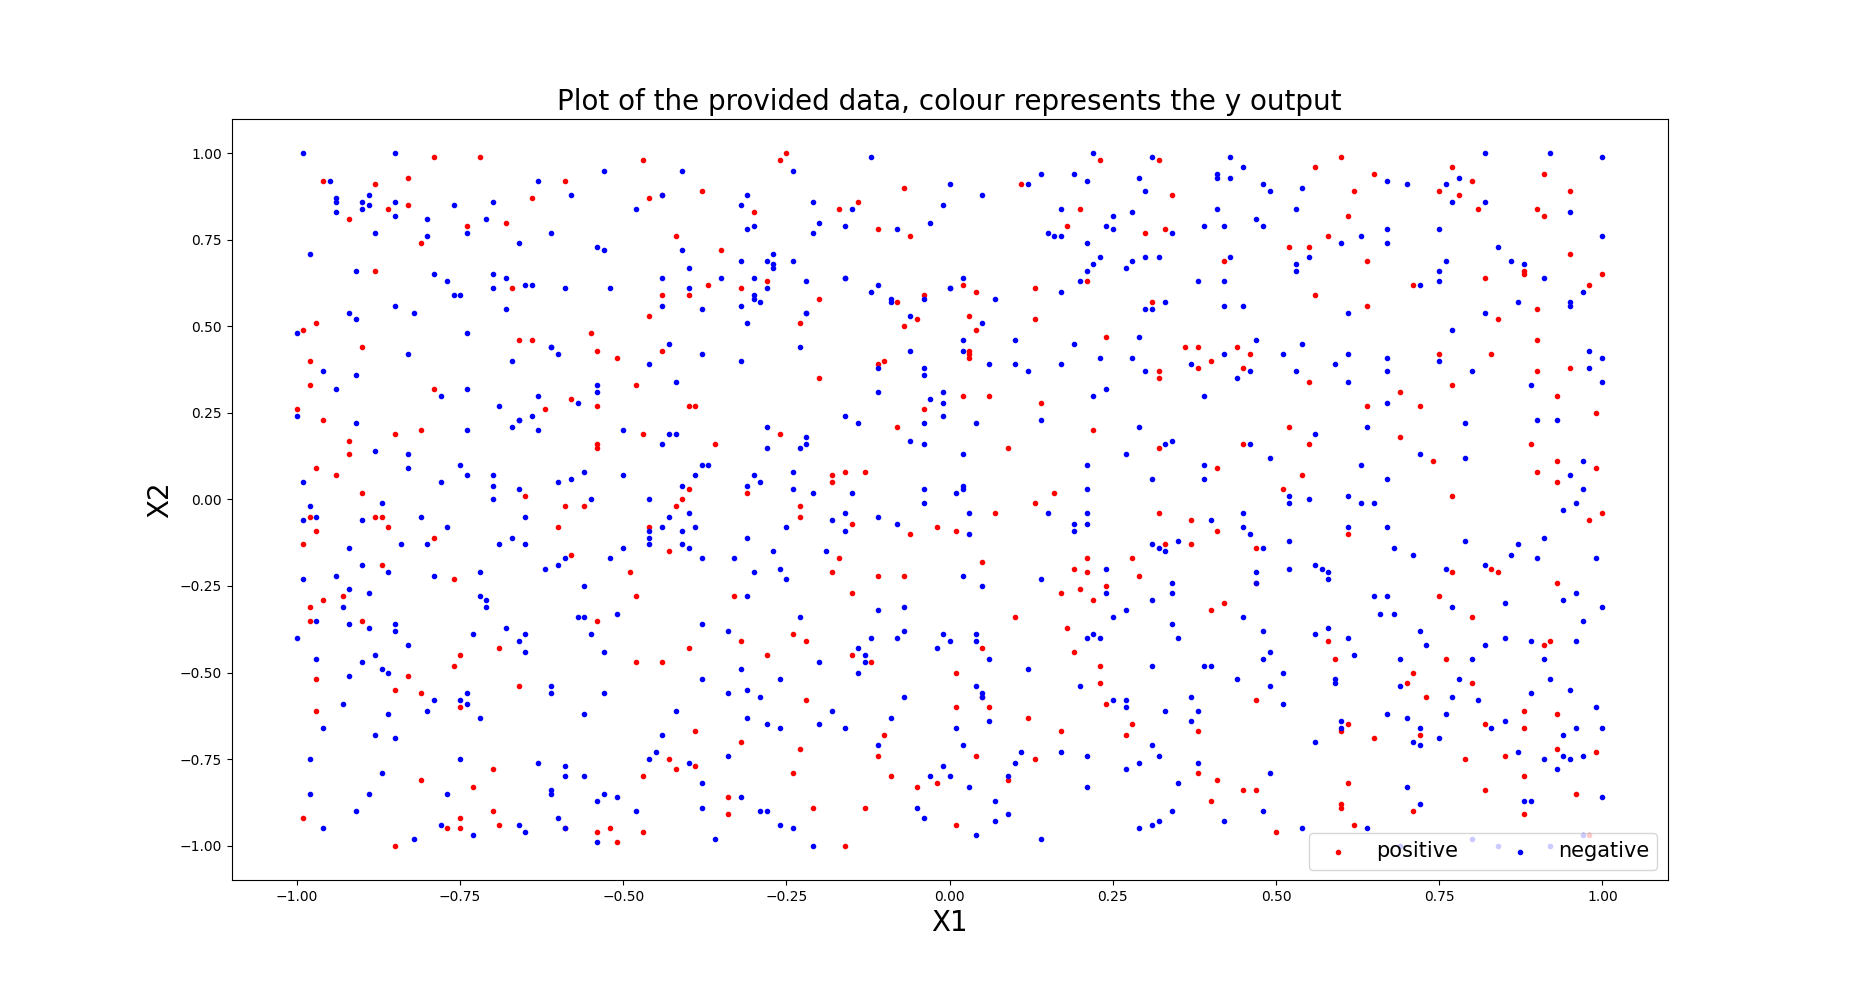
\includegraphics[scale=0.15]{Figure_2.png}}   
    \fbox{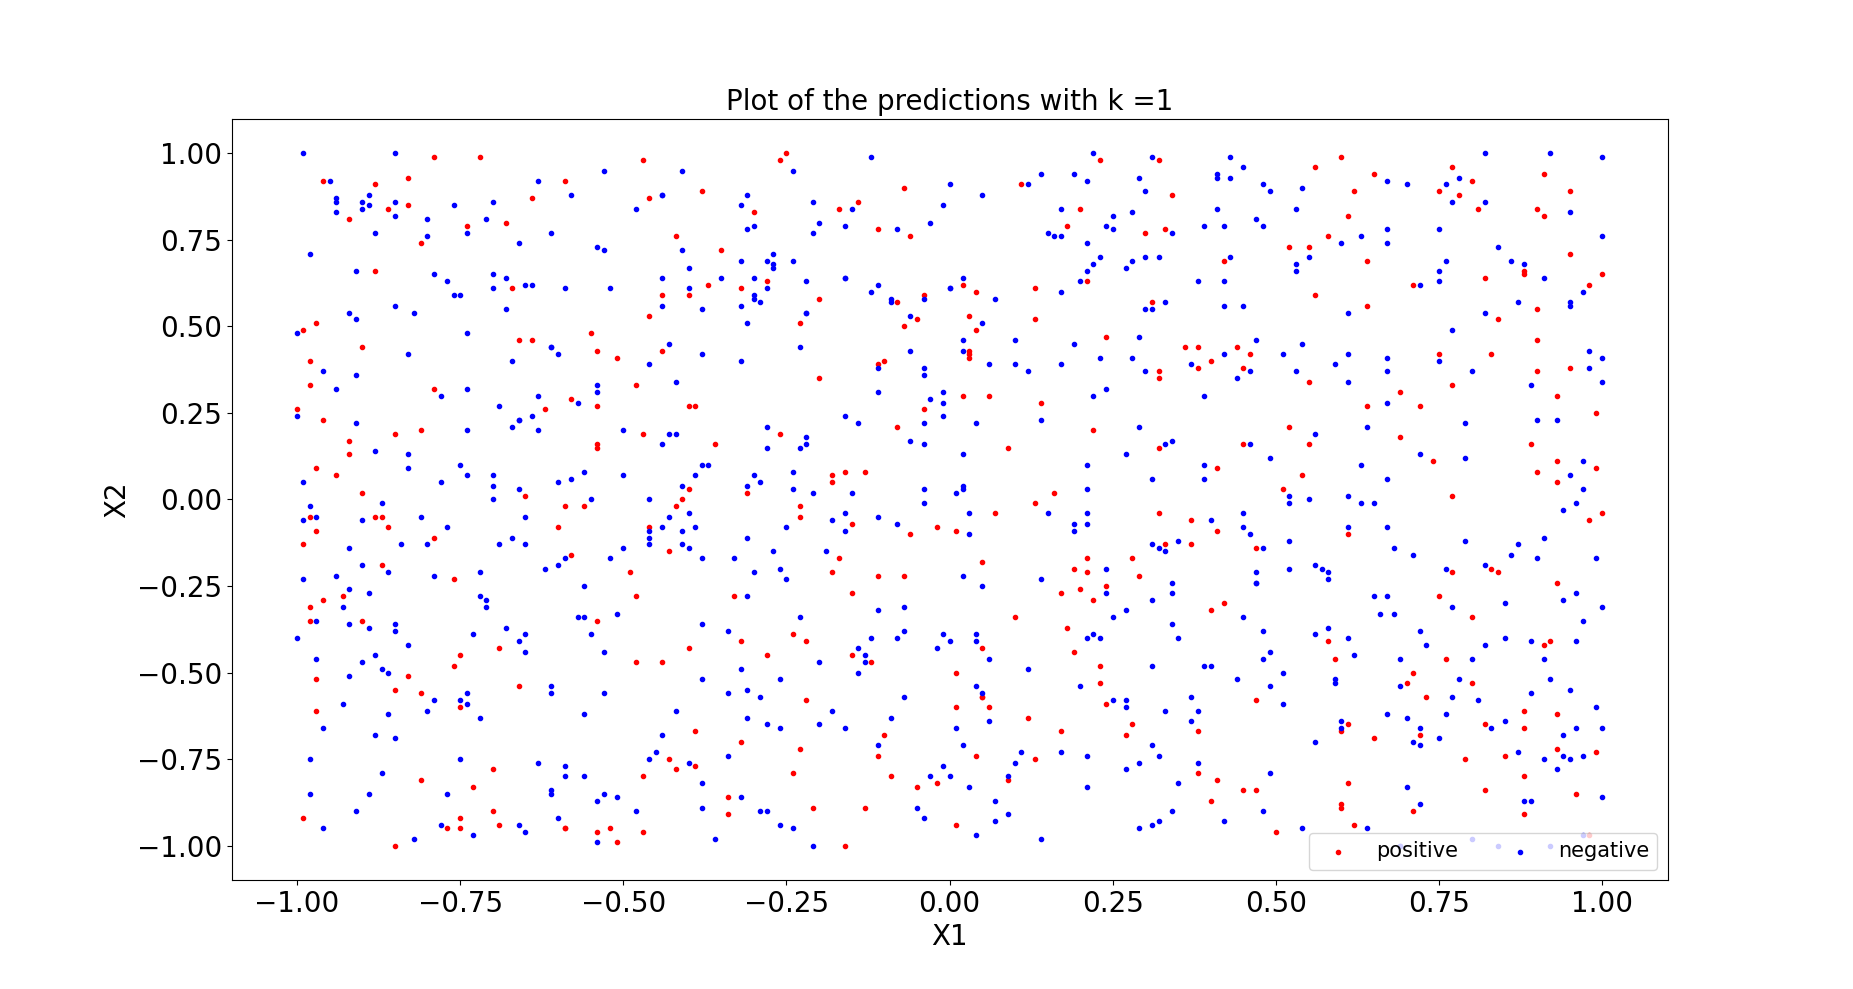
\includegraphics[scale=0.15]{ds_2_pred_knn_1.png}}   
    \fbox{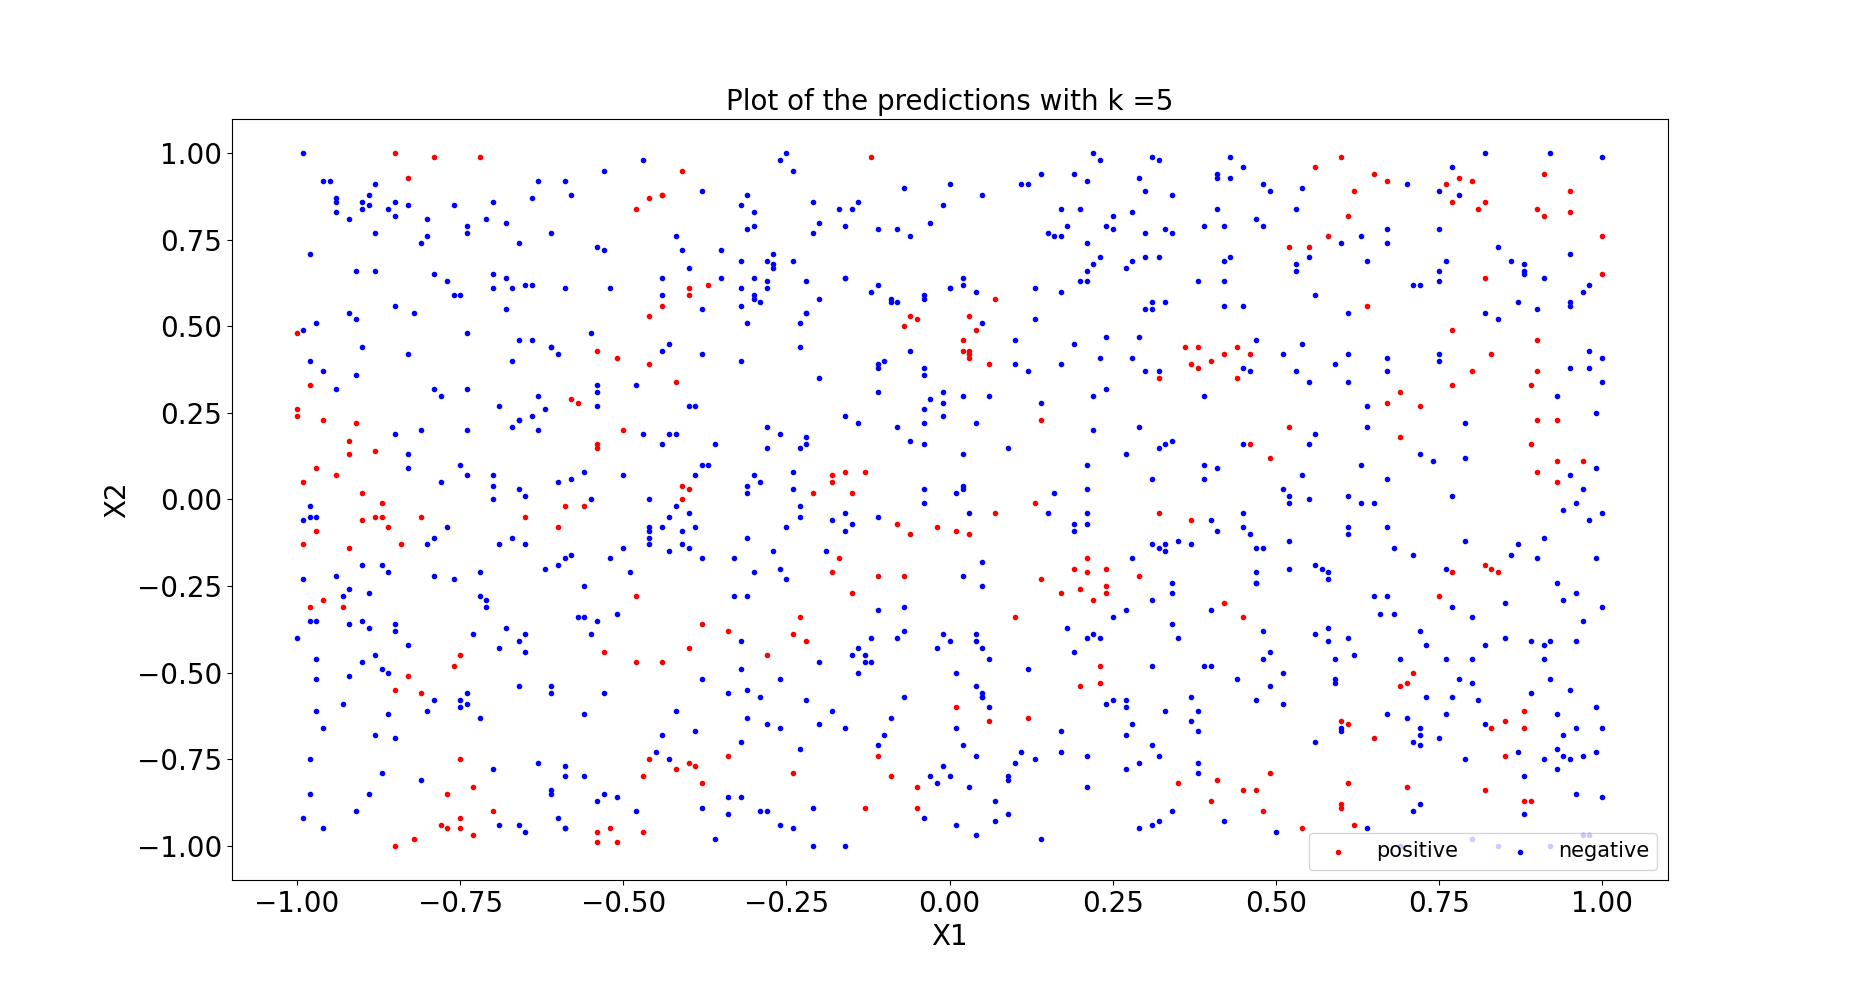
\includegraphics[scale=0.15]{ds_2_pred_knn_5.png}}
    \fbox{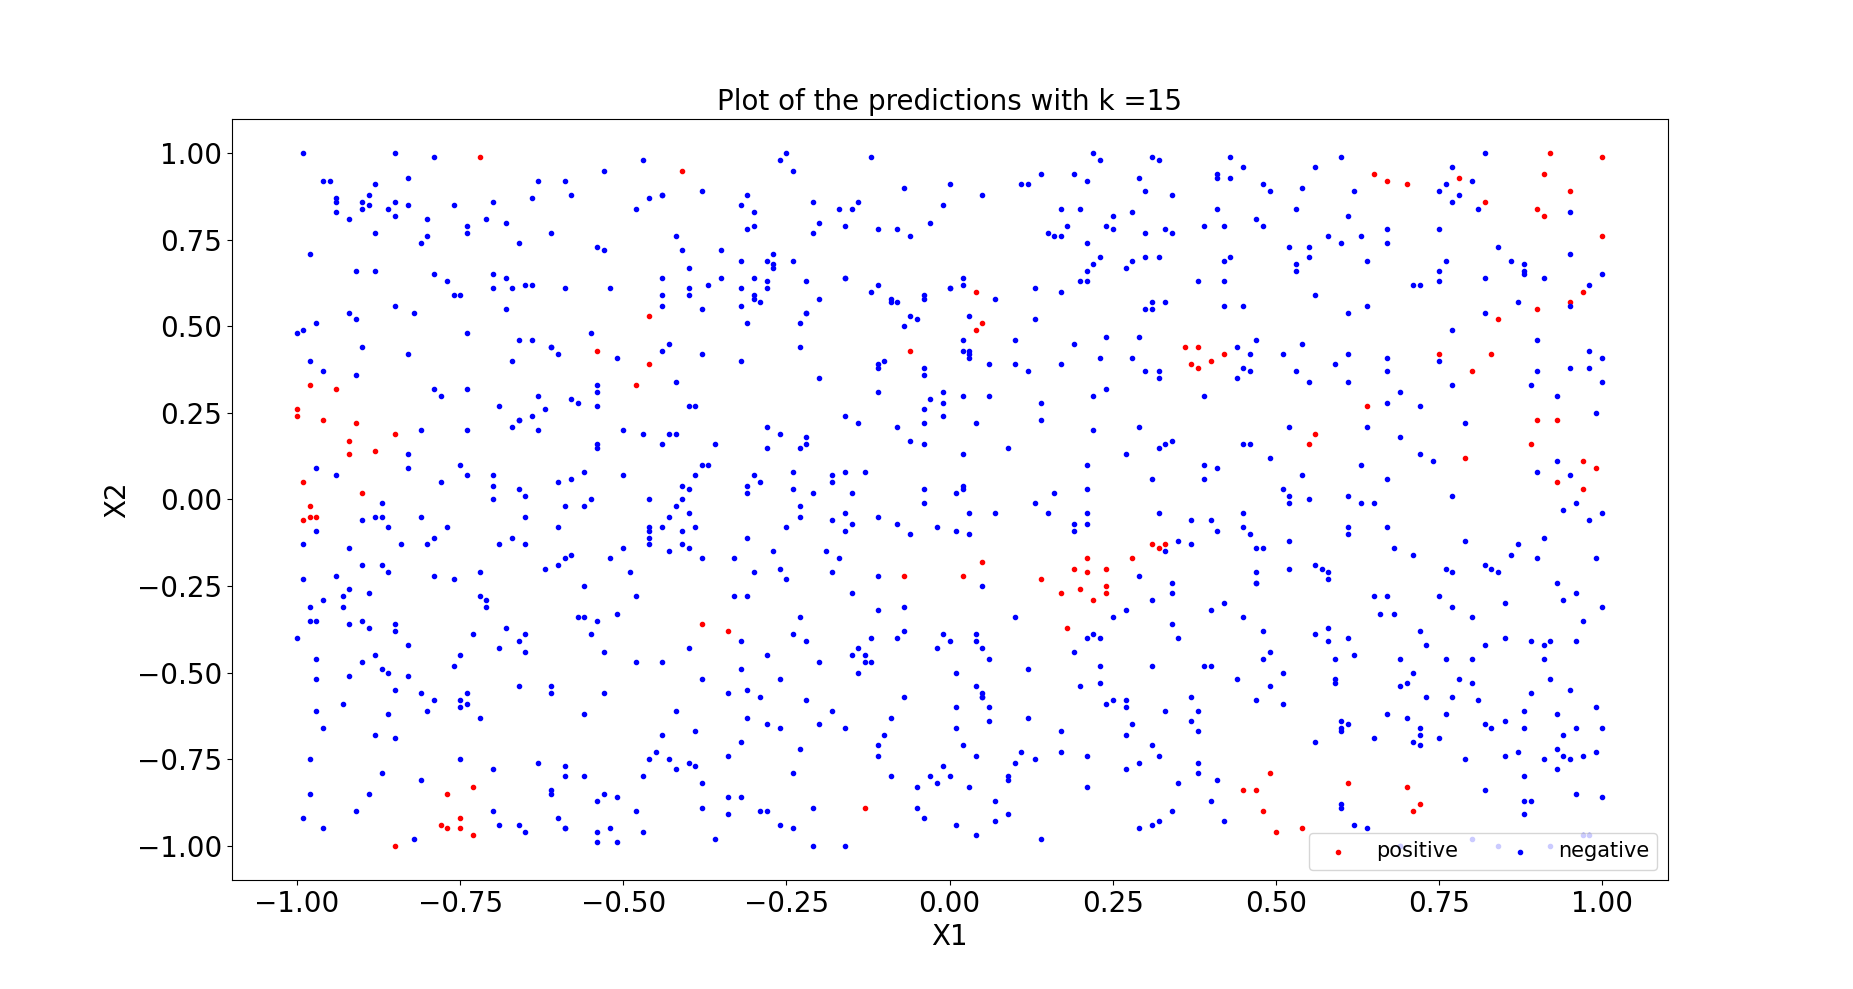
\includegraphics[scale=0.15]{ds_2_pred_knn_15.png}}
\end{figure}
We notice a similar pattern as we did in question i.
We can notice that the model with $ k = 1 $ behaves better and that the
higher the k value the more clusters of predictions are formed and we can clearly
see from the original data that this pattern is not desired.
\par
Let's now consider the possibility of potentially augmenting the feature for that kNN model.
Using the same method of cross validation for a large range of polynomial degrees, we obtain the following plot.
Note that this plot used the previously selected value $ k = 1 $.

\begin{center}
    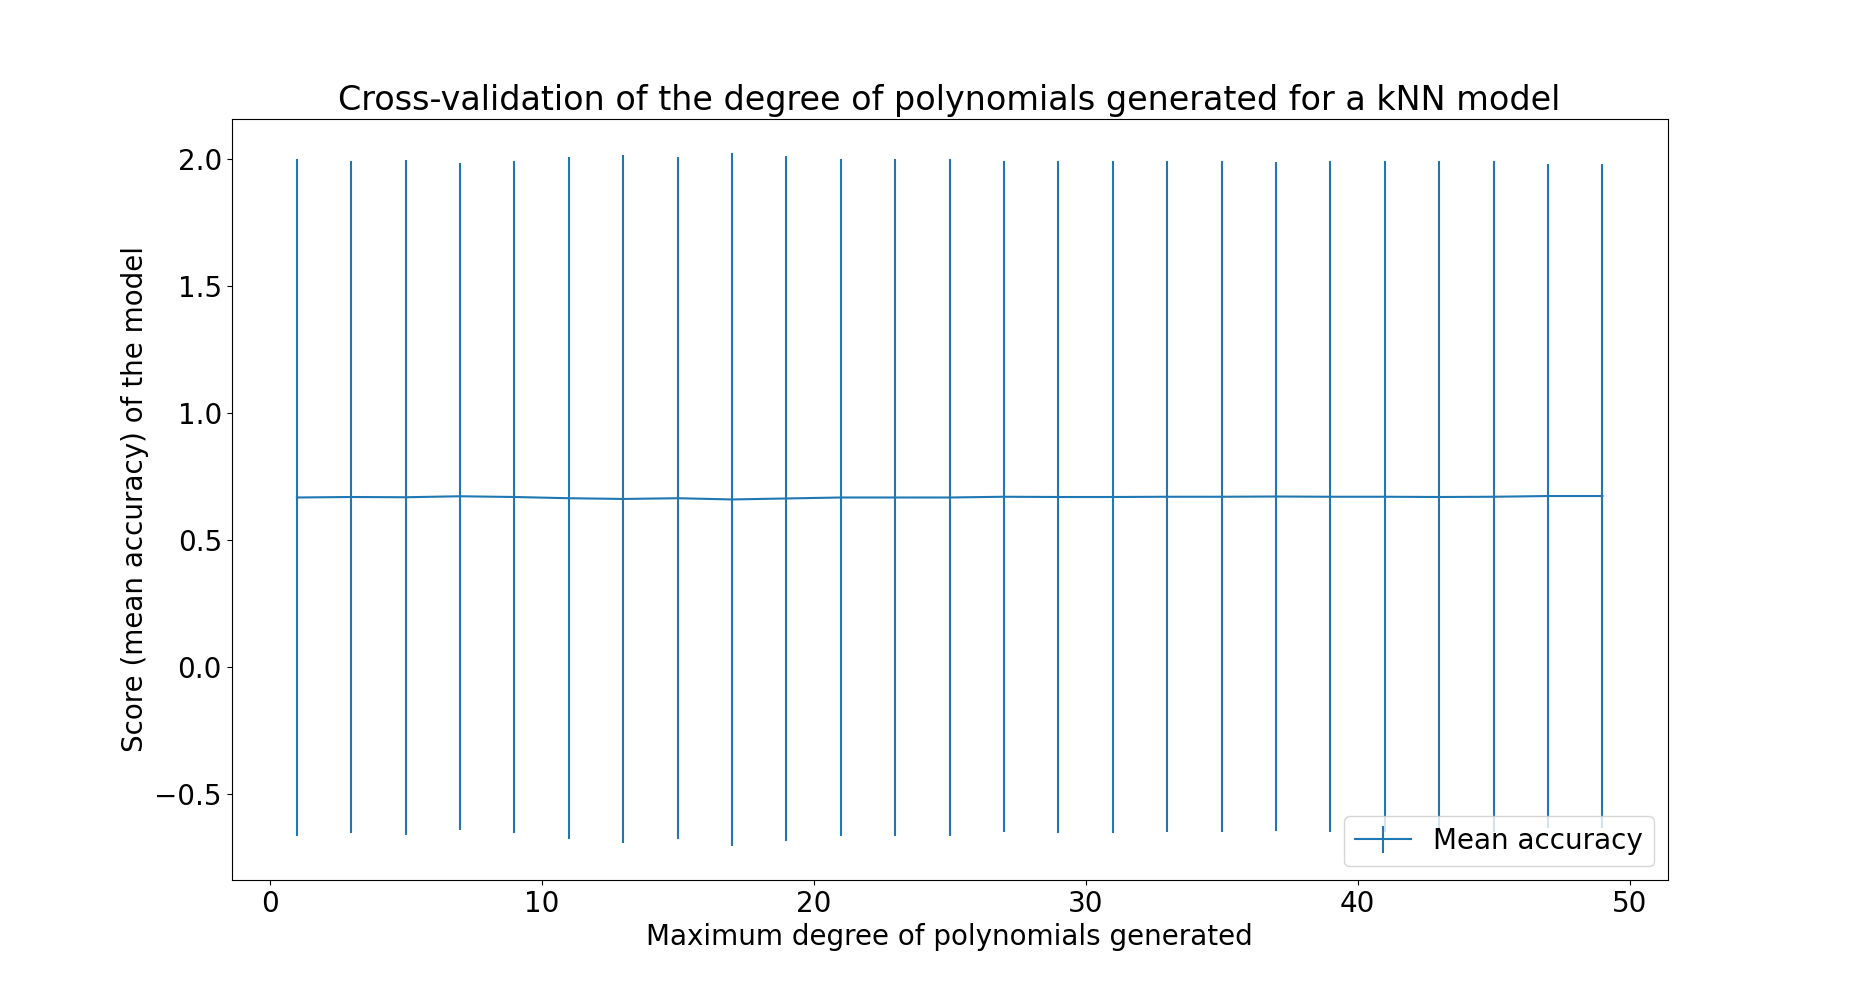
\includegraphics[scale=0.25]{ds_2_knn_d_cv.png}
\end{center}
\vspace{5mm} %5mm vertical space
We notice absolutely no advantage with our selected k value to augment the 2 features we have.
Both the accuracy and mean squared error remains roughly the same.

\subsection*{Part c}
For this part, I will train 4 models using the parameters that we identified in previous questions.
That is:
\begin{itemize}
    \item Logistic Regression (L2) model, with C = 1 and non augmented features.
    \item kNN Model, with k = 1 and the default provided features.
    \item Most frequent value model, a model which always predicts the most common output.
    \item Random model, a model which always predicts a random output.
  \end{itemize}


Once again the implementation is the same as we've seen in question i, let's plot the tables:
\par
\vspace{5mm} %5mm vertical space
ROC Table for the kNN model, using k = 1 and the default features from the dataset:
\par
\vspace{5mm} %5mm vertical space
\begin{tabularx}{0.8\textwidth} { 
    | >{\raggedright\arraybackslash}X 
    | >{\centering\arraybackslash}X 
    | >{\raggedleft\arraybackslash}X | }
    \hline
     & Predicted positive & Predicted negative \\
    \hline
    True positive & 681 & 2 \\
   \hline
   True negative  & 2 & 353 \\
  \hline
\end{tabularx}
\par
We notice straight away that the predictions are close to perfect, with only 4 predictions
not being correct.
\par
\vspace{5mm} %5mm vertical space
ROC Table for the Logistic Regression model, using $ C = 1 $.
\par
\vspace{5mm} %5mm vertical space
\begin{tabularx}{0.8\textwidth} { 
    | >{\raggedright\arraybackslash}X 
    | >{\centering\arraybackslash}X 
    | >{\raggedleft\arraybackslash}X | }
    \hline
     & Predicted positive & Predicted negative \\
    \hline
    True positive & 683 & 0 \\
   \hline
   True negative  & 355 & 0 \\
  \hline
\end{tabularx}
\par
We notice that predictions here are always positive, thus we only see
true positives and false positives. This models predictions are accurate roughly over 2/3rd of
the time. We can notice that this is the same model as a most frequent value model.
\par
\vspace{5mm} %5mm vertical space
ROC Table for the Random model:
\par
\vspace{5mm} %5mm vertical space
\begin{tabularx}{0.8\textwidth} { 
    | >{\raggedright\arraybackslash}X 
    | >{\centering\arraybackslash}X 
    | >{\raggedleft\arraybackslash}X | }
    \hline
     & Predicted positive & Predicted negative \\
    \hline
    True positive & 336 & 347 \\
   \hline
   True negative  & 184 & 171 \\
  \hline
\end{tabularx}
\par
Here we notice that the values are a bit all over the place, this makes sense as our model
is truly random thus it is expected.
\par
\vspace{5mm} %5mm vertical space
ROC Table for the Most frequent value model:
\par
\vspace{5mm} %5mm vertical space
\begin{tabularx}{0.8\textwidth} { 
    | >{\raggedright\arraybackslash}X 
    | >{\centering\arraybackslash}X 
    | >{\raggedleft\arraybackslash}X | }
    \hline
     & Predicted positive & Predicted negative \\
    \hline
    True positive & 683 & 0 \\
   \hline
   True negative  & 355 & 0 \\
  \hline
\end{tabularx}
\par
For this final model we only find true positives and true negatives,
this makes sense as our model predicts the most common value (which in this case is
positive). We find that roughly over 2/3rds of predictions are correct. We can also notice that
this is the exact same table as for out Logistic Regression model!

\subsection*{Part d}
Using the exact same method as explained previously, we obtain the following ROC plot for our 4 models:
\begin{center}
    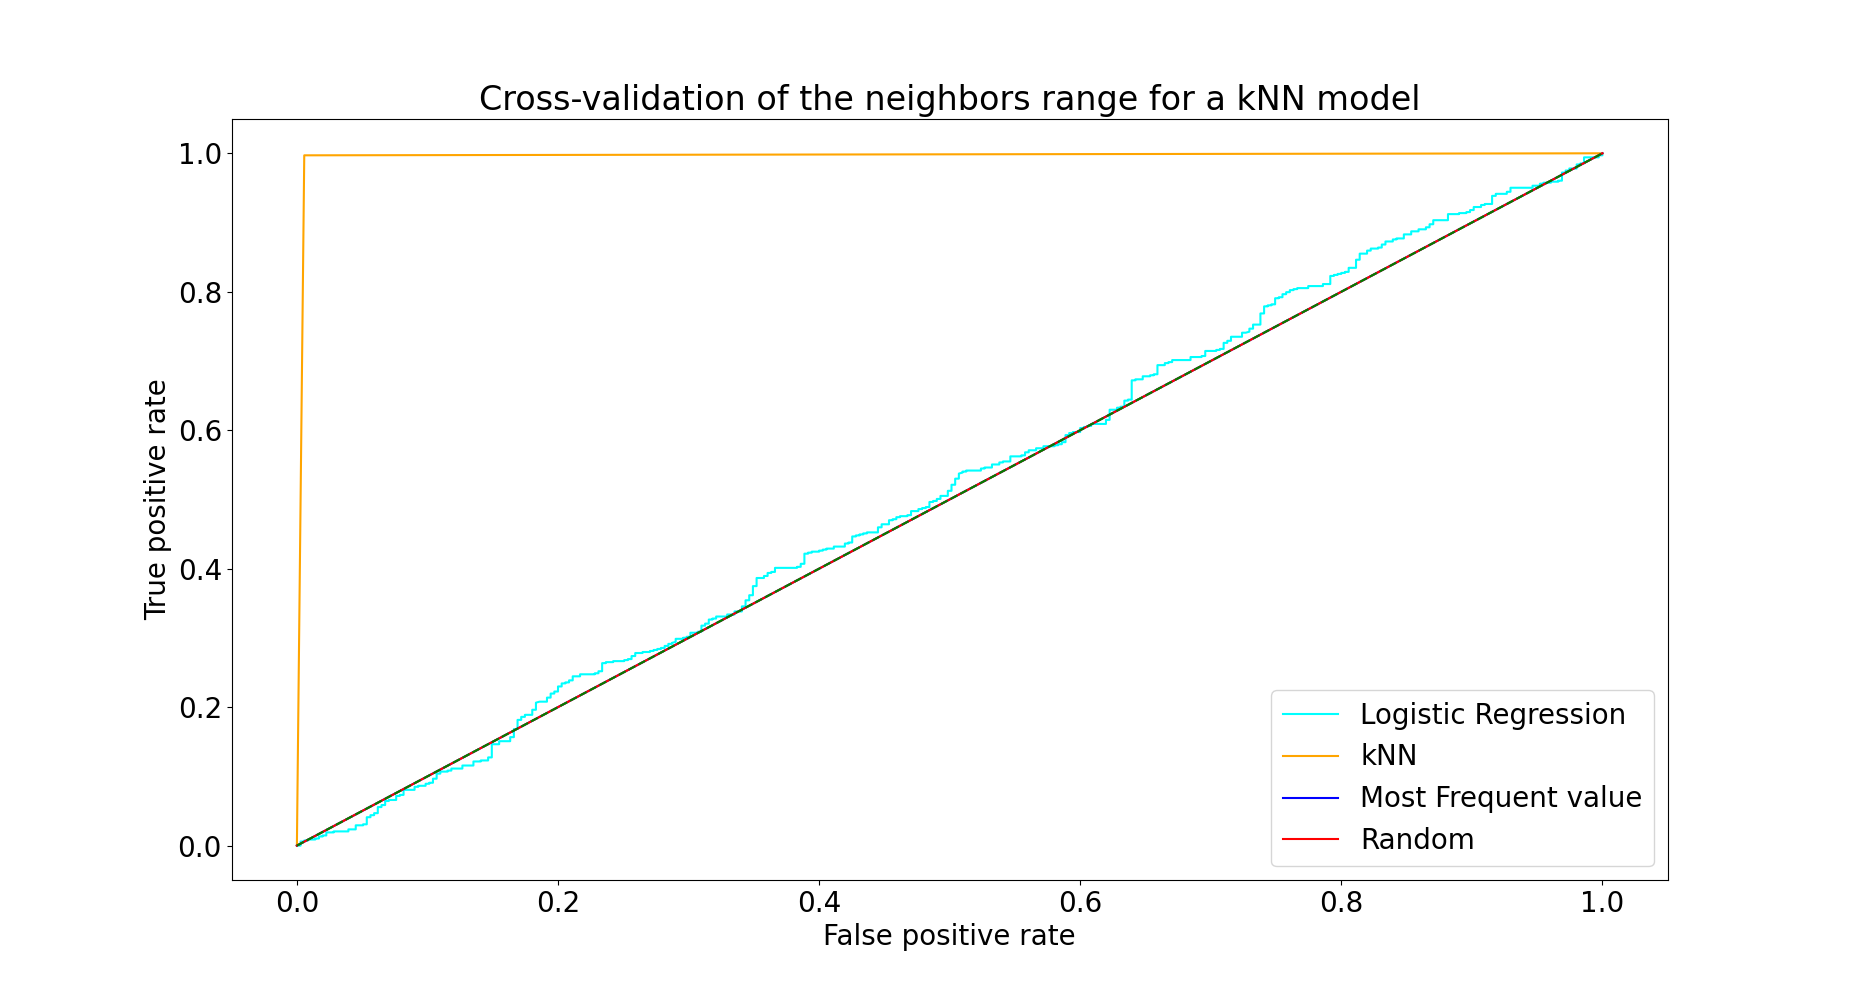
\includegraphics[scale=0.25]{roc_2.png}
\end{center}
\vspace{5mm} %5mm vertical space

We can clearly see that the kNN model is doing quite well. The other 3 models are quite similar in their plot
with the expection of the logistic regression where we can see some variation.

\subsection*{Part e}
Let's start with the random model, we can clearly see that its confusion matrix is by far
the worst out of all of our models, that is because the outputs are compeletely unpredictable so let's move on.
\par
The most frequent value baseline model is the exact same as the logistic model in this case in terms
of our confusion matrix. We find that the ROC curve for the logistic model varies slightly, usually towards a higher value of
true positive rate but ocasionally down too, while the baseline model stays straight throughout.
\par
The clear winner here is the kNN model which has clearly the best confusion matrix with only 4 predictions being false and
and ROC curve which is optimal.

\section*{Appendix}
Code for question i and ii is the same but using a different dataset and using different parameters,
to avoid this report getting too long I wil simply put the code once.
\par

Part a:
\begin{lstlisting}[language=Python]    
from sklearn.metrics import mean_squared_error
from sklearn.preprocessing import PolynomialFeatures
from sklearn.model_selection import KFold
from sklearn.linear_model import LogisticRegression
import numpy as np
import pandas as pd
import matplotlib.pyplot as plt

# Read in data
df = pd.read_csv("week4.csv", comment='#')
X1 = df.iloc[:, 0]
X2 = df.iloc[:, 1]
X = np.column_stack((X1, X2))
y = np.array(df.iloc[:, 2])

# Plotting the data alone
fig = plt.figure()
ax = fig.add_subplot(111)
neg = plt.scatter(X1[y < 0], X2[y < 0], 
                        color='red', marker=".")
pos = plt.scatter(X1[y > 0], X2[y > 0], 
                        color='blue', marker=".")
ax.set_ylabel("X2", fontsize=20)
ax.set_xlabel("X1", fontsize=20)
ax.set_title(
    "Plot of the provided data, colour represents "+
                        "the y output", fontsize=20)
plt.rc('font', size=20)
plt.legend((neg, pos), ["positive", "negative"],
            scatterpoints=1,
            loc='lower right',
            ncol=2,
            fontsize=15)

# Compute a simple logistic regression with 
#varying degrees of polynomials.
degrees = range(1, 10)
scores = []
temp = []
for degree in degrees:
    # Generate new features
    poly = PolynomialFeatures(degree)
    X_poly = poly.fit_transform(X)
    # Train the model
    model = LogisticRegression(penalty='l2')
                                .fit(X_poly, y)
    # Keep the score of the model
    scores.append(model.score(X_poly, y))
    temp.append(mean_squared_error(y, 
                        model.predict(X_poly)))


# Plot the scores for each model.
fig = plt.figure()
plt.rc('font', size=20)
ax = fig.add_subplot(111)
ax.errorbar(degrees, scores,
        label='Mean accuracy',yerr=temp)
ax.set_ylabel("Score (mean accuracy) of the model")
ax.set_xlabel("Maximum degree of polynomials generated")
ax.set_title(
    "Cross-validation of the degree of polynomials" +
            "generated for a Logistic Regression model")
ax.legend(loc='lower right')

# Use interesting degrees to plot the predictions
for degree in [1, 2, 10]:
    poly = PolynomialFeatures(degree)
    X_poly = poly.fit_transform(X)
    model = LogisticRegression(solver='liblinear',
                        penalty='l2').fit(X_poly, y)
    y_pred = model.predict(X_poly)
    # Plt the predictions
    fig = plt.figure()
    ax = fig.add_subplot(111)
    neg = plt.scatter(X1[y_pred < 0], X2[y_pred < 0],
                                color='red', marker=".")
    pos = plt.scatter(X1[y_pred > 0], X2[y_pred > 0],
                                color='blue', marker=".")
    ax.set_ylabel("X2", fontsize=20)
    ax.set_xlabel("X1", fontsize=20)
    ax.set_title(
    "Plot of the predictions with polynomial features "+
                    "up to " + str(degree), fontsize=20)
    plt.rc('font', size=20)
    plt.legend((neg, pos), ["positive", "negative"],
                scatterpoints=1,
                loc='lower right',
                ncol=2,
                fontsize=15)


# cross validate C value
C_values = range(1, 30, 1)
scores = []
temp = []
for C in C_values:
    poly = PolynomialFeatures(2)
    X_poly = poly.fit_transform(X)
    model = LogisticRegression(C=C).fit(X_poly, y)
    scores.append(model.score(X_poly, y))
    temp.append(mean_squared_error(y,
                        model.predict(X_poly)))

# Plot the scores for each model.
fig = plt.figure()
plt.rc('font', size=20)
ax = fig.add_subplot(111)
ax.errorbar(C_values, scores, label='Mean accuracy',
                                        yerr=temp)
ax.set_ylabel("Score (mean accuracy) of the model")
ax.set_xlabel("C")
ax.set_title(
    "Cross-validation of the l2 penalty term C " +
                    "for a Logistic Regression model")
ax.legend(loc='lower right')

# Plot predictions with some C values
C_values = [1, 8, 35]
scores = []
for C in C_values:
    poly = PolynomialFeatures(2)
    X_poly = poly.fit_transform(X)
    model = LogisticRegression(
        solver='liblinear', penalty='l2', C=C)
                                .fit(X_poly, y)
    # Plt the predictions
    fig = plt.figure()
    ax = fig.add_subplot(111)
    neg = plt.scatter(X1[y_pred < 0], X2[y_pred < 0],
                            color='red', marker=".")
    pos = plt.scatter(X1[y_pred > 0], X2[y_pred > 0],
                            color='blue', marker=".")
    ax.set_ylabel("X2", fontsize=20)
    ax.set_xlabel("X1", fontsize=20)
    ax.set_title(
        "Plot of the predictions with C =" + str(C),
                                        fontsize=20)
    plt.rc('font', size=20)
    plt.legend((neg, pos), ["positive", "negative"],
                scatterpoints=1,
                loc='lower right',
                ncol=2,
                fontsize=15)
plt.show()
\end{lstlisting}
\par

Part b
\begin{lstlisting}[language=Python]    
from sklearn.neighbors import KNeighborsClassifier
import numpy as np
import pandas as pd
import matplotlib.pyplot as plt
from sklearn.preprocessing import PolynomialFeatures
from sklearn.metrics import mean_squared_error

# Read in data
df = pd.read_csv("week4.csv", comment='#')
X1 = df.iloc[:, 0]
X2 = df.iloc[:, 1]
X = np.column_stack((X1, X2))
y = np.array(df.iloc[:, 2])

neighbors_range = range(1, 20, 1)
scores = []
temp = []
for n in neighbors_range:
    model = KNeighborsClassifier(
        n_neighbors=n, weights='uniform').fit(X, y)
    scores.append(model.score(X, y))
    temp.append(mean_squared_error(y, model.predict(X)))

# Plot the scores for each model.
fig = plt.figure()
plt.rc('font', size=20)
ax = fig.add_subplot(111)
ax.errorbar(neighbors_range, scores,
                    label='Mean accuracy', yerr=temp)
ax.set_ylabel("Score (mean accuracy) of the model")
ax.set_xlabel("k")
ax.set_title(
    "Cross-validation of the neighbors" +
                    "range for a kNN model")
ax.legend(loc='lower right')

# Plot predictions with some k values
K_values = [1, 5, 15]
scores = []
for K in K_values:
    model = KNeighborsClassifier(
        n_neighbors=K, weights='uniform').fit(X, y)
    y_pred = model.predict(X)
    # Plt the predictions
    fig = plt.figure()
    ax = fig.add_subplot(111)
    neg = plt.scatter(X1[y_pred < 0], X2[y_pred < 0],
                                color='red', marker=".")
    pos = plt.scatter(X1[y_pred > 0], X2[y_pred > 0],
                                color='blue', marker=".")
    ax.set_ylabel("X2", fontsize=20)
    ax.set_xlabel("X1", fontsize=20)
    ax.set_title(
        "Plot of the predictions with k =" +
                            str(K), fontsize=20)
    plt.rc('font', size=20)
    plt.legend((neg, pos), ["positive", "negative"],
                scatterpoints=1,
                loc='lower right',
                ncol=2,
                fontsize=15)


# Compute a simple knn model with varying
# degrees of polynomials.
degrees = range(1, 50, 2)
scores = []
temp = []
for degree in degrees:
    poly = PolynomialFeatures(degree)
    X_poly = poly.fit_transform(X)
    model = KNeighborsClassifier(
        n_neighbors=K, weights='uniform').fit(X_poly, y)
    scores.append(model.score(X_poly, y))
    temp.append(mean_squared_error(y, 
                        model.predict(X_poly)))

# Plot the scores for each model.
fig = plt.figure()
plt.rc('font', size=20)
ax = fig.add_subplot(111)
ax.errorbar(degrees, scores, label='Mean accuracy',
                                        yerr=temp)
ax.set_ylabel("Score (mean accuracy) of the model")
ax.set_xlabel("Maximum degree of polynomials generated")
ax.set_title(
    "Cross-validation of the degree of" +
            "polynomials generated for a kNN model")
ax.legend(loc='lower right')

plt.show()
\end{lstlisting}
\par

Part c
\begin{lstlisting}[language=Python]
from sklearn.metrics import roc_curve
from sklearn.neighbors import KNeighborsClassifier
import numpy as np
import pandas as pd
import matplotlib.pyplot as plt
from sklearn.preprocessing import PolynomialFeatures
from sklearn.linear_model import LogisticRegression
from sklearn.metrics import confusion_matrix
import statistics
import random
from sklearn.dummy import DummyClassifier

# Read in data
df = pd.read_csv("week4.csv", comment='#')
X1 = df.iloc[:, 0]
X2 = df.iloc[:, 1]
X = np.column_stack((X1, X2))
y = np.array(df.iloc[:, 2])
# Compute polynomials
poly = PolynomialFeatures(2)
X_poly = poly.fit_transform(X)

print("printing in order: tn, fp, fn, tp")

# Train our models
knnModel = KNeighborsClassifier(
    n_neighbors=1, weights='uniform').fit(X, y)
knn_pred = knnModel.predict(X)
tn, fp, fn, tp = confusion_matrix(y, knn_pred).ravel()
print("knn model", tn, fp, fn, tp)

lgModel = LogisticRegression(C=8).fit(X_poly, y)
lg_pred = lgModel.predict(X_poly)
tn, fp, fn, tp = confusion_matrix(y, lg_pred).ravel()
print("logistic regression model: ", tn, fp, fn, tp)

randomModel = DummyClassifier(strategy="uniform")
mostFreqModel = DummyClassifier(strategy="most_frequent")

randomModel.fit(X, y)
mostFreqModel.fit(X, y)

# Random
rqndom_pred = randomModel.predict(X)
tn, fp, fn, tp = confusion_matrix(y, rqndom_pred).ravel()
print("random model: ", tn, fp, fn, tp)

# Uniform
most_freq_pred = mostFreqModel.predict(X)
tn, fp, fn, tp = confusion_matrix(y,
                    most_freq_pred).ravel()
print("most freq value model: ", tn, fp, fn, tp)

# logistic roc
fpr, tpr, _ = roc_curve(y, 
                lgModel.decision_function(X_poly))
# knn roc
knn_proba = knnModel.predict_proba(X)
knn_fpr, knn_tpr, thresh = roc_curve(y, knn_proba[:, 1])

# most freq val roc
most_freq_proba = mostFreqModel.predict_proba(X)
most_freq_fpr, most_freq_tpr, thresh = roc_curve(y,
                            most_freq_proba[:, 1])

# random roc
rand_proba = randomModel.predict_proba(X)
rand_fpr, rand_tpr, thresh = roc_curve(y,
                                rand_proba[:, 1])


fig = plt.figure()
plt.rc('font', size=20)
ax = fig.add_subplot(111)
ax.plot(fpr, tpr, color='cyan')
ax.plot(knn_fpr, knn_tpr, color='orange')
ax.plot(most_freq_fpr, most_freq_tpr, color='blue')
ax.plot(rand_fpr, rand_tpr, color='red')
ax.plot([0, 1], [0, 1], color='green', linestyle='--')
ax.set_ylabel('True positive rate')
ax.set_xlabel('False positive rate')
ax.set_title(
    "Cross-validation of the neighbors" +
                    "range for a kNN model")
plt.legend(["Logistic Regression", "kNN",
            "Most Frequent value", "Random"])
plt.show()

\end{lstlisting}
\end{document}
